\documentclass[12pt,a4paper,oneside]{report} 

% Load math packages before style to avoid \Bbbk conflict with newpxmath
\usepackage{amsmath,amssymb,amsthm}

% Language and type configuration (UBB template)
\usepackage[language=english, type=bachelor]{style}

% Cleveref must be loaded after hyperref (which is in style.sty)
\usepackage[capitalize,noabbrev]{cleveref}

% PDF metadata and hyperref configuration (most is in style.sty)
\hypersetup{
    pdftitle={Hybrid Post-Quantum Key Exchange for WireGuard: Integrating ML-KEM into a Production Rust Userspace Implementation},
    pdfauthor={Mihai-Cristian Farcaș},
    pdfsubject={Bachelor's Thesis - Computer Science},
    pdfkeywords={WireGuard, Post-Quantum Cryptography, ML-KEM, FIPS 203, Hybrid Key Exchange, Noise Protocol, Rust, BoringTun},
}

\begin{document}

\specialization{Computer Science}
\title{Hybrid Post-Quantum Key Exchange for WireGuard: Integrating ML-KEM into a Production Rust Userspace Implementation}   
\author{Mihai-Cristian Farcaș}
\supervisor{Sergiu Adrian Dărăbanț}

\maketitle

% Blank page after title
\newpage
\thispagestyle{empty}
\mbox{}
\newpage

% Front matter with roman numerals
\pagenumbering{roman}
\setcounter{page}{1}

% Abstract
\chapter*{Abstract}
\addcontentsline{toc}{chapter}{Abstract}
\markboth{ABSTRACT}{ABSTRACT}

WireGuard is now the dominant modern VPN protocol, valued for its small codebase, strong cryptography, and high performance. Its key exchange, however, relies entirely on X25519, which Shor's algorithm will break once a cryptographically relevant quantum computer exists. Under the harvest-now-decrypt-later threat model, adversaries may already be recording WireGuard-encrypted traffic today for future decryption, making migration urgent rather than speculative.

\vspace{0.5cm}

NIST finalized FIPS 203 in August 2024, standardizing ML-KEM (Module Lattice-based Key Encapsulation Mechanism), derived from CRYSTALS-Kyber. This thesis integrates ML-KEM-768 alongside X25519 into WireGuard's Noise IK handshake, producing a hybrid post-quantum key exchange. The implementation targets BoringTun, Cloudflare's production Rust userspace WireGuard, and is deployable without kernel modifications. A simpler baseline that injects ML-KEM-derived keying material into WireGuard's existing preshared-key (PSK) slot is also implemented as a lower bound on engineering effort. Both approaches are evaluated on Apple Silicon (M4) and ARM (Raspberry Pi 5 / Cortex-A76), measuring handshake latency and packet size overhead. An informal security argument shows the hybrid construction to be secure as long as at least one of X25519 or ML-KEM remains unbroken, and that it provides per-session forward secrecy that the PSK-slot approach cannot match. To our knowledge, this is the first FIPS 203-compliant hybrid WireGuard implementation built on a production Rust codebase.

\vspace{1cm}

\noindent\textbf{Keywords:} Post-Quantum Cryptography, WireGuard, ML-KEM, FIPS 203, Hybrid Key Exchange, Noise Protocol, Rust, BoringTun

% Table of Contents
\cleardoublepage
\tableofcontents

% List of Figures
\cleardoublepage
\listoffigures

% List of Tables
\cleardoublepage
\listoftables

% Main content with arabic numerals
\cleardoublepage
\pagenumbering{arabic}
\setcounter{page}{1}

\chapter{Introduction}
\label{chap:introduction}

Public-key cryptography underpins virtually all secure communication on the internet. VPN tunnels, TLS handshakes, SSH connections: they all depend on the computational hardness of problems like integer factorization and the elliptic-curve discrete logarithm, problems that classical computers cannot efficiently solve at cryptographic parameter sizes. This assumption has held for decades, but it will not hold forever.

Peter Shor's 1994 polynomial-time quantum algorithm~\cite{shor1994algorithms} solves both integer factorization and the discrete logarithm problem, which means a sufficiently large fault-tolerant quantum computer would break RSA and elliptic-curve cryptography in polynomial time. The security community has been aware of this since the 1990s, but for most of that time quantum hardware was too primitive to pose a real threat. That is changing. Current estimates put the cost of factoring RSA-2048 at roughly millions of physical qubits with today's error-correction techniques~\cite{gidney2021factor}, and hardware roadmaps from IBM, Google, and others suggest that scale could be reached within the next decade or two.

In response, NIST launched its Post-Quantum Cryptography (PQC) Standardization Project in 2016, finalizing the first round of standards in August 2024: FIPS 203 (ML-KEM, for key encapsulation)~\cite{fips203}, FIPS 204 (ML-DSA, for digital signatures), and FIPS 205 (SLH-DSA, hash-based signatures). For VPN key exchange, ML-KEM is the directly relevant standard. NIST has also set a hard timeline: classical key exchange algorithms are to be deprecated by 2030 and disallowed entirely by 2035~\cite{nistir8547}.

WireGuard is among the most important migration targets. Since Donenfeld introduced it in 2017~\cite{donenfeld2017wireguard}, it has largely replaced IPsec and OpenVPN as the go-to VPN protocol, thanks to its small codebase, strong performance, and easy auditability. It ships in the Linux kernel, runs on every major operating system, and is deployed at scale by Cloudflare, Mullvad, NordVPN, Tailscale, and many enterprises. But WireGuard's cryptographic design is deliberately opinionated: a fixed cipher suite with no negotiation. This rigidity is a security advantage (cipher agility has been a recurring source of vulnerabilities in TLS and IPsec), but it makes migration harder, since there is no built-in way to swap in a different key exchange algorithm.

WireGuard does, however, provide two natural handles for post-quantum augmentation. The first is the preshared-key (PSK) slot, a 256-bit symmetric key that is mixed into the handshake's key derivation chain. If a post-quantum KEM is used out-of-band to establish this PSK, the resulting handshake is quantum-resistant against passive adversaries, at the cost of requiring separate key distribution infrastructure. The second approach is to modify the Noise IK handshake itself, embedding ML-KEM operations alongside the existing X25519 exchange so that both shared secrets contribute to the final session key in every handshake. The latter is what we call the full hybrid approach.

This thesis makes four contributions. It implements a PSK-slot baseline: a small CLI tool that performs ML-KEM-768 key encapsulation between two peers out-of-band and feeds the resulting 256-bit key into BoringTun's~\cite{boringtun} preshared\_key field. It then implements the full hybrid: a modified BoringTun whose handshake module runs both X25519 and ML-KEM-768 in every handshake, mixing both shared secrets into the Noise chaining key via HMAC-BLAKE2s, with no changes to the data-transport phase. Both implementations are evaluated on Apple Silicon (M4) and Raspberry Pi 5 hardware, measuring handshake overhead and packet sizes. Finally, a security analysis compares the two approaches and discusses where each one fits in practice.

The rest of the thesis is structured as follows. Chapter~\ref{chap:background} covers the relevant background: the quantum threat, WireGuard, the Noise framework, and ML-KEM. Chapter~\ref{chap:related_work} surveys prior work on post-quantum WireGuard. Chapter~\ref{chap:problem} states the research question. Chapters~\ref{chap:design} and~\ref{chap:implementation} describe the design and implementation, respectively. Chapter~\ref{chap:security} analyzes security properties. Chapter~\ref{chap:evaluation} reports the evaluation results. Chapter~\ref{chap:discussion} discusses tradeoffs, deployment considerations, and future work, and Chapter~\ref{chap:conclusions} concludes.

\section*{Declaration of Generative AI and AI-Assisted Technologies in the Writing Process}

During the preparation of this work I used Claude (Anthropic's large language model) via the Claude Code CLI tool for these purposes: as a coding assistant while implementing the hybrid handshake and PSK-slot tool in Rust, for designing and interpreting the benchmarks, and as an editor to tighten the thesis prose and catch places where the written descriptions had drifted from what the code actually does. After using this tool, I reviewed and edited the content as needed and take full responsibility for the content of the thesis.

\chapter{Background}
\label{chap:background}

\section{The Quantum Threat and Public-Key Cryptography}

All widely deployed public-key cryptography relies on computational hardness assumptions. RSA depends on the difficulty of integer factorization; Diffie-Hellman and its elliptic-curve variants (including X25519, as used in WireGuard) depend on the discrete logarithm problem. No polynomial-time classical algorithm is known for any of these at cryptographic parameter sizes, and for decades that has been enough.

Shor's algorithm~\cite{shor1994algorithms} upends this. A fault-tolerant quantum computer with enough qubits can solve both integer factorization and discrete logarithm in polynomial time, an exponential speedup over the best classical approaches. Concretely, such a machine could derive an X25519 private key from the corresponding public key and reconstruct any session key derived from it. Gidney and Eker\aa~\cite{gidney2021factor} estimate that RSA-2048 could be factored with roughly 20 million noisy qubits in a matter of hours.

What makes this urgent is the harvest-now-decrypt-later (HNDL) attack model. An adversary who lacks a quantum computer today can still passively record encrypted traffic --- WireGuard handshakes, transport data, all of it --- and store it cheaply. Once a sufficiently powerful quantum computer is available, the adversary recovers the X25519 private keys from the stored public keys, reconstructs the ephemeral shared secrets, and decrypts everything. The uncomfortable implication is that traffic encrypted today with classical-only key exchange may already be compromised in a meaningful sense, even though the quantum computers needed to exploit it do not yet exist.

Symmetric cryptography, by contrast, is largely safe. Grover's algorithm provides only a quadratic speedup for brute-force search, effectively halving key lengths: AES-256 retains 128 bits of security against quantum adversaries, which is still more than adequate. ChaCha20-Poly1305, BLAKE2s, and the HMAC-based key derivation used by WireGuard are similarly unaffected. The migration problem is confined to the asymmetric key exchange layer.

NIST's response was a structured standardization effort that produced ML-KEM for key encapsulation, ML-DSA for signatures, and SLH-DSA for hash-based signatures. The accompanying transition timeline is concrete: classical key exchange (RSA, ECDH, ECDSA) is to be deprecated after 2030 and disallowed after 2035~\cite{nistir8547}. Organizations handling data that must remain confidential past 2035 face an even tighter deadline, since that data is already at risk from HNDL collection if protected only by classical key exchange today.

\section{WireGuard: Protocol Design and Architecture}

WireGuard~\cite{donenfeld2017wireguard} is a layer-3 VPN protocol built around a small set of modern cryptographic primitives and a deliberately minimal state machine. Donenfeld's design philosophy favours conservatism: a fixed cipher suite with no algorithm negotiation, a single round-trip handshake, and fewer than 4,000 lines of code in the reference implementation.

The core cryptographic design uses Trevor Perrin's Noise Protocol Framework~\cite{noise-protocol} for the handshake, specifically the IK pattern, combined with X25519 for Diffie-Hellman key exchange, HKDF~\cite{rfc5869} for key derivation, ChaCha20-Poly1305 for authenticated encryption of transport data, and BLAKE2s for hashing.

WireGuard's networking model is built around a concept called cryptokey routing: each peer is identified by a 32-byte Curve25519 public key, and the interface maintains a mapping from public keys to allowed IP address ranges. This means that IP-level authentication is cryptographically derived — any packet arriving on a WireGuard interface has a reliably authenticated source IP, provided the underlying session was established correctly.

The handshake produces a 1-RTT session. The initiator sends a first message that authenticates both the initiator's identity (via the static public key) and commits an ephemeral Curve25519 key. The responder verifies the initiator's identity, generates its own ephemeral key, and sends a response message. After the response is processed, both parties independently derive the same pair of symmetric session keys using HKDF. Transport data subsequently flows in UDP packets using ChaCha20-Poly1305 with a nonce counter.

\begin{figure}[!htbp]
    \centering
    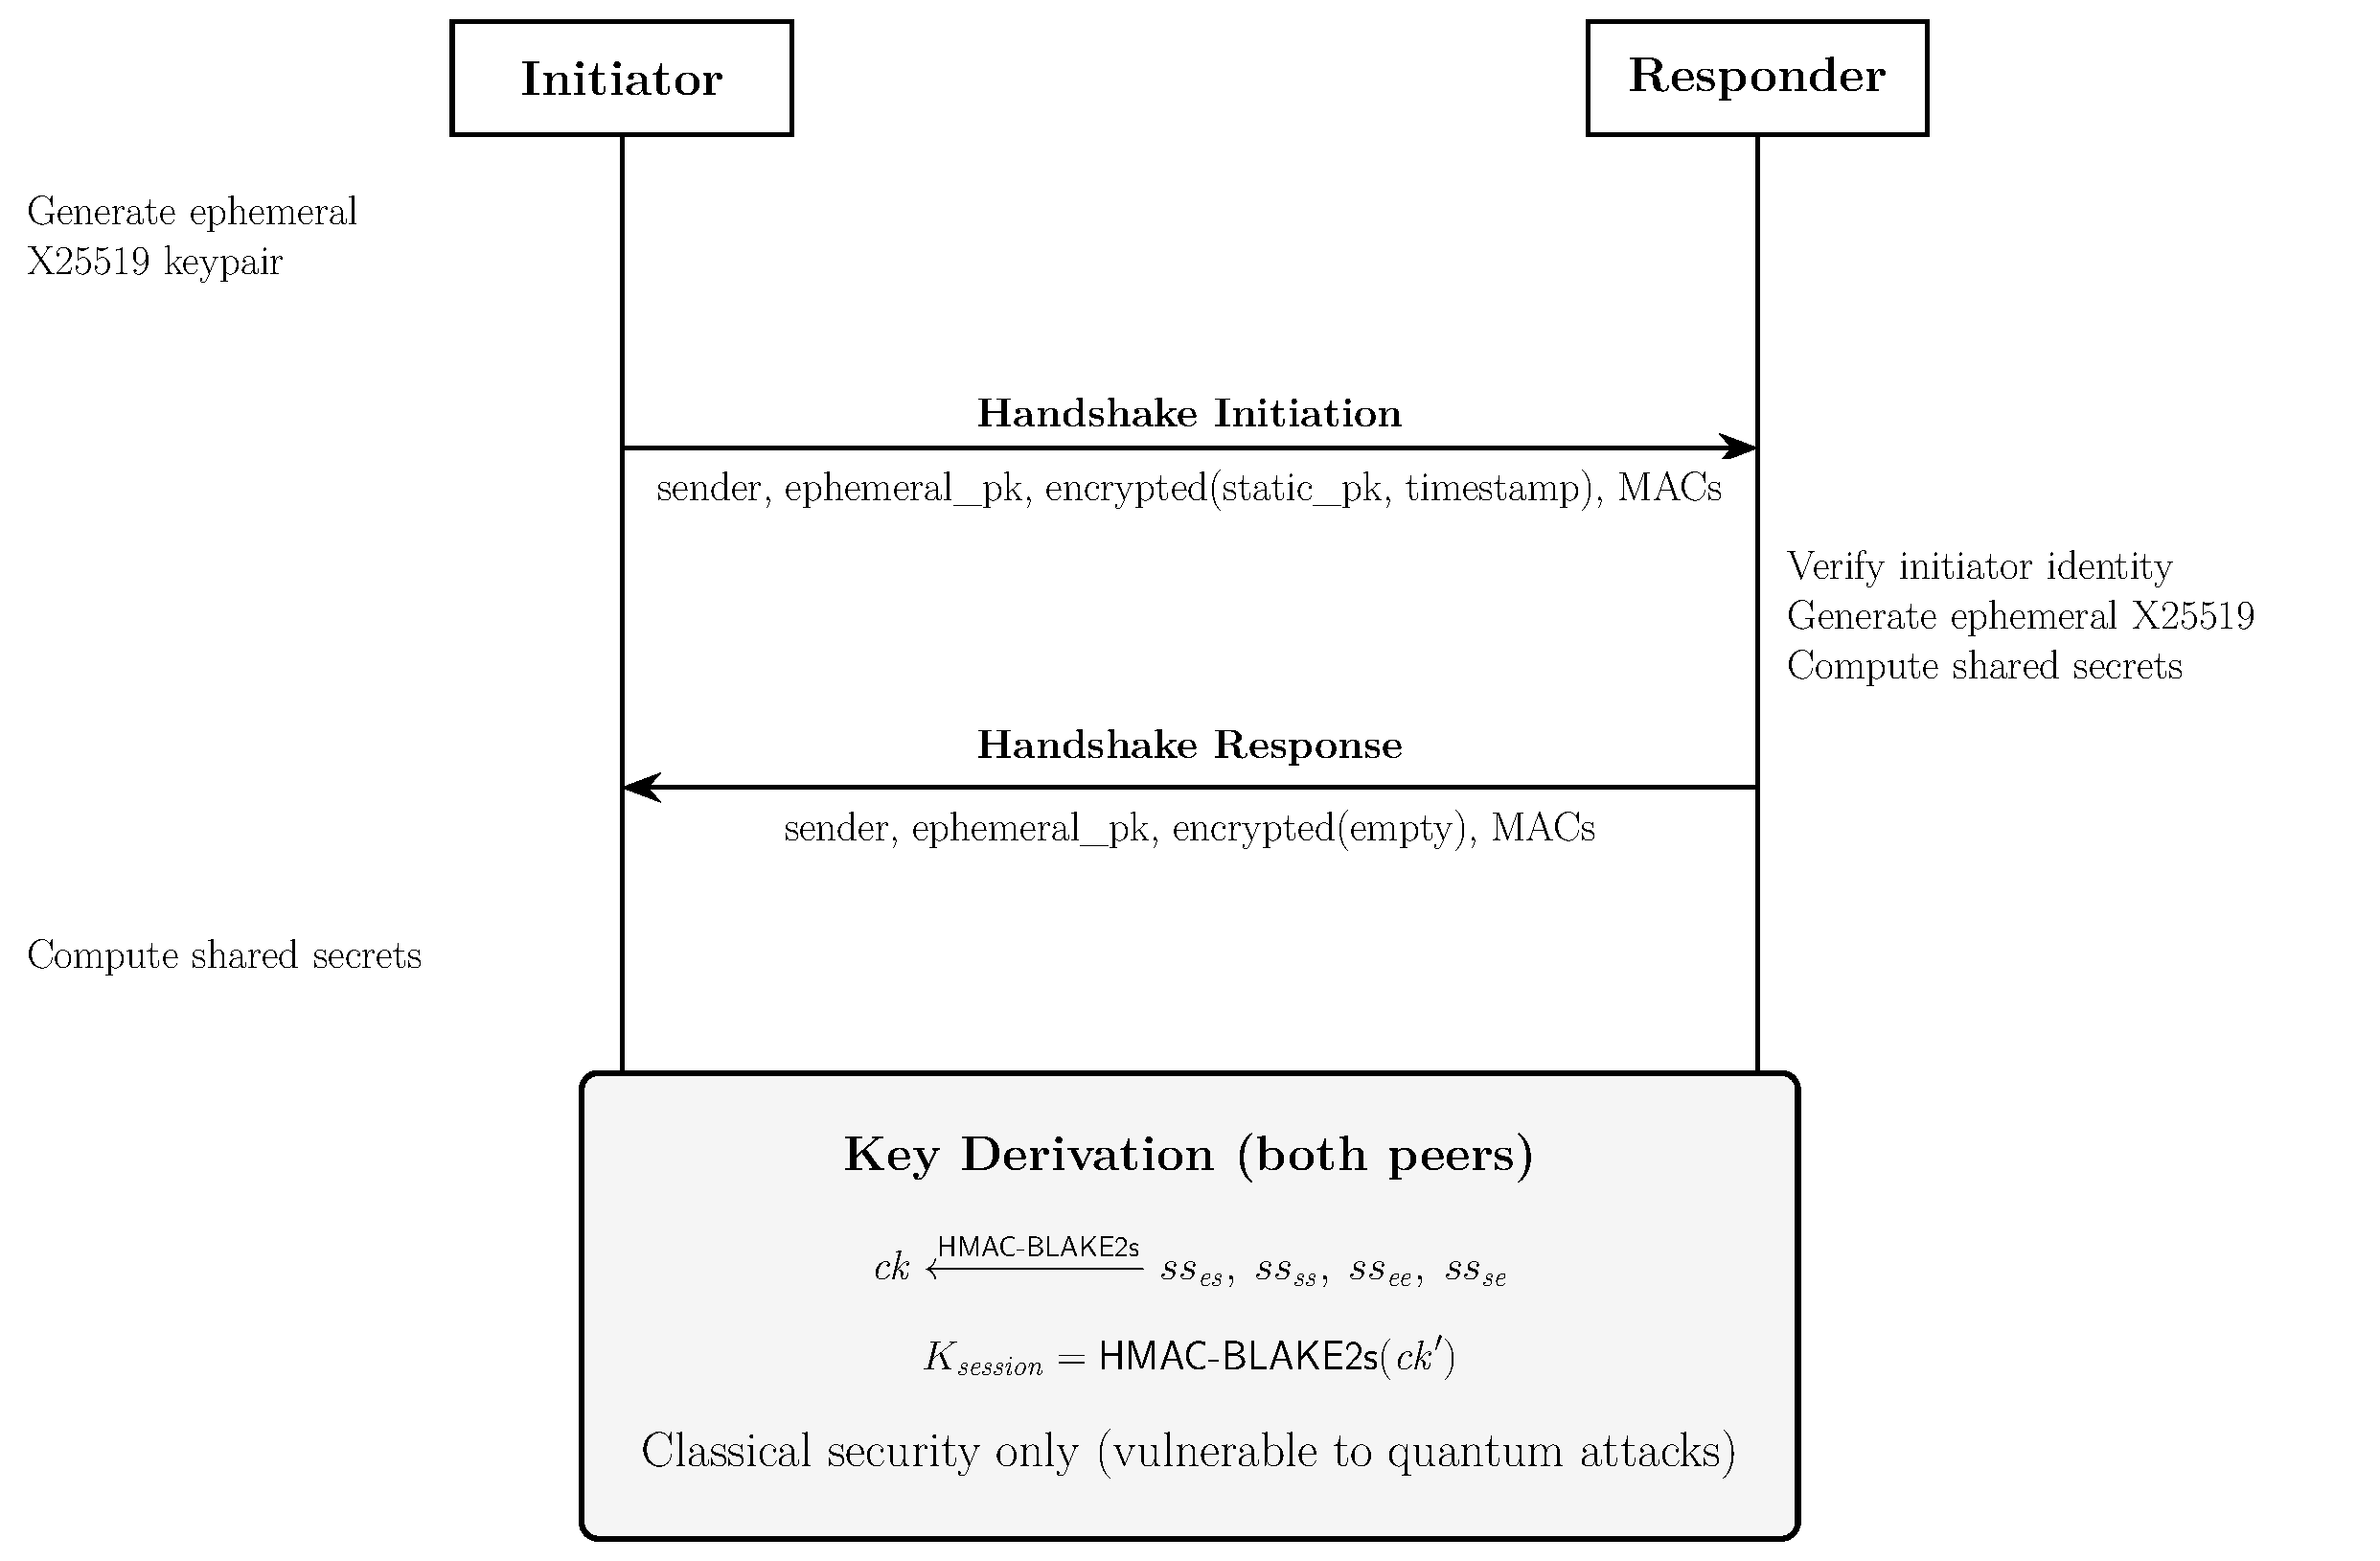
\includegraphics[width=\textwidth]{figures/fig_vanilla_handshake.pdf}
    \caption{Vanilla WireGuard Handshake (Noise IK pattern).}
    \label{fig:vanilla_handshake}
\end{figure}

WireGuard's timer state machine handles session lifecycle automatically: sessions rekey after 120 seconds or after 2\textsuperscript{60} transport messages, whichever comes first. All ephemeral keys and intermediate cryptographic material are zeroed from memory after use.

WireGuard also has unusually strong denial-of-service resistance. The responder never allocates state for unauthenticated packets, which makes it invisible to port scanners and limits the impact of resource-exhaustion attacks. When under load, a cookie mechanism lets the responder push work back to the initiator.

Performance-wise, WireGuard significantly outperforms legacy VPN protocols. Donenfeld's benchmarks show roughly 0.403ms ping times and the ability to saturate a gigabit Ethernet link, beating both OpenVPN and IPsec in AES-GCM and ChaCha20 modes.

\subsection{The PSK Slot}

WireGuard includes an optional pre-shared symmetric key (PSK) feature, added specifically to provide a measure of post-quantum protection. When configured, this 256-bit symmetric key is mixed into the HKDF key derivation chain during the handshake, adding a layer of symmetric-key cryptography on top of the X25519 exchange. The design intent is that even if a quantum computer eventually breaks X25519, an attacker who did not also obtain the PSK at the time of the session cannot decrypt the traffic.

The PSK mechanism was explicitly designed as a transitional measure for ``the extremely paranoid.'' Its limitations are structural: the PSK is a long-lived static value, not an ephemeral secret, so it does not provide forward secrecy for the quantum-resistant component. If the PSK itself is compromised — whether through theft, misconfiguration, or an insider — all sessions protected by it are retrospectively vulnerable. Distribution and rotation of PSKs also requires an out-of-band channel, shifting operational complexity to deployment teams.

\section{The Noise Protocol Framework}

Noise, designed by Trevor Perrin, is a framework for building authenticated key exchange protocols from a small set of cryptographic patterns. A Noise pattern specifies the sequence of messages exchanged between an initiator and a responder, along with the Diffie-Hellman operations performed at each step and the order in which public keys become known to each party.

WireGuard uses the IK pattern, named for how each party's static key is handled: \emph{I} for the initiator's static, which is transmitted \emph{immediately} during the handshake (encrypted, so passive eavesdroppers cannot see it), and \emph{K} for the responder's static, which is \emph{known} to the initiator beforehand. The pattern provides a one-round-trip mutually authenticated key exchange and identity hiding for the initiator's static against passive observers.

Noise protocols maintain two running state values: a chaining key (ck) and a handshake hash (h). Each DH operation, public key transmission, and encrypted payload is mixed into these values via HKDF and BLAKE2s, building a transcript hash that cryptographically binds all handshake messages together. The session keys at the end of the handshake are derived from the final value of ck.

The main difficulty in migrating Noise to post-quantum cryptography is that its design is deeply tied to the algebraic properties of Diffie-Hellman. DH provides non-interactive key exchange: the initiator can compute $g^{ab}$ from the responder's public key $g^b$ and its own private key $a$, and vice versa, without any interaction. KEMs work differently: one party generates a ciphertext that encapsulates a secret to a specific public key, and only the holder of the corresponding private key can decapsulate it. This asymmetry means the handshake flow needs to be reworked when KEMs are introduced.

\begin{figure}[!htbp]
    \centering
    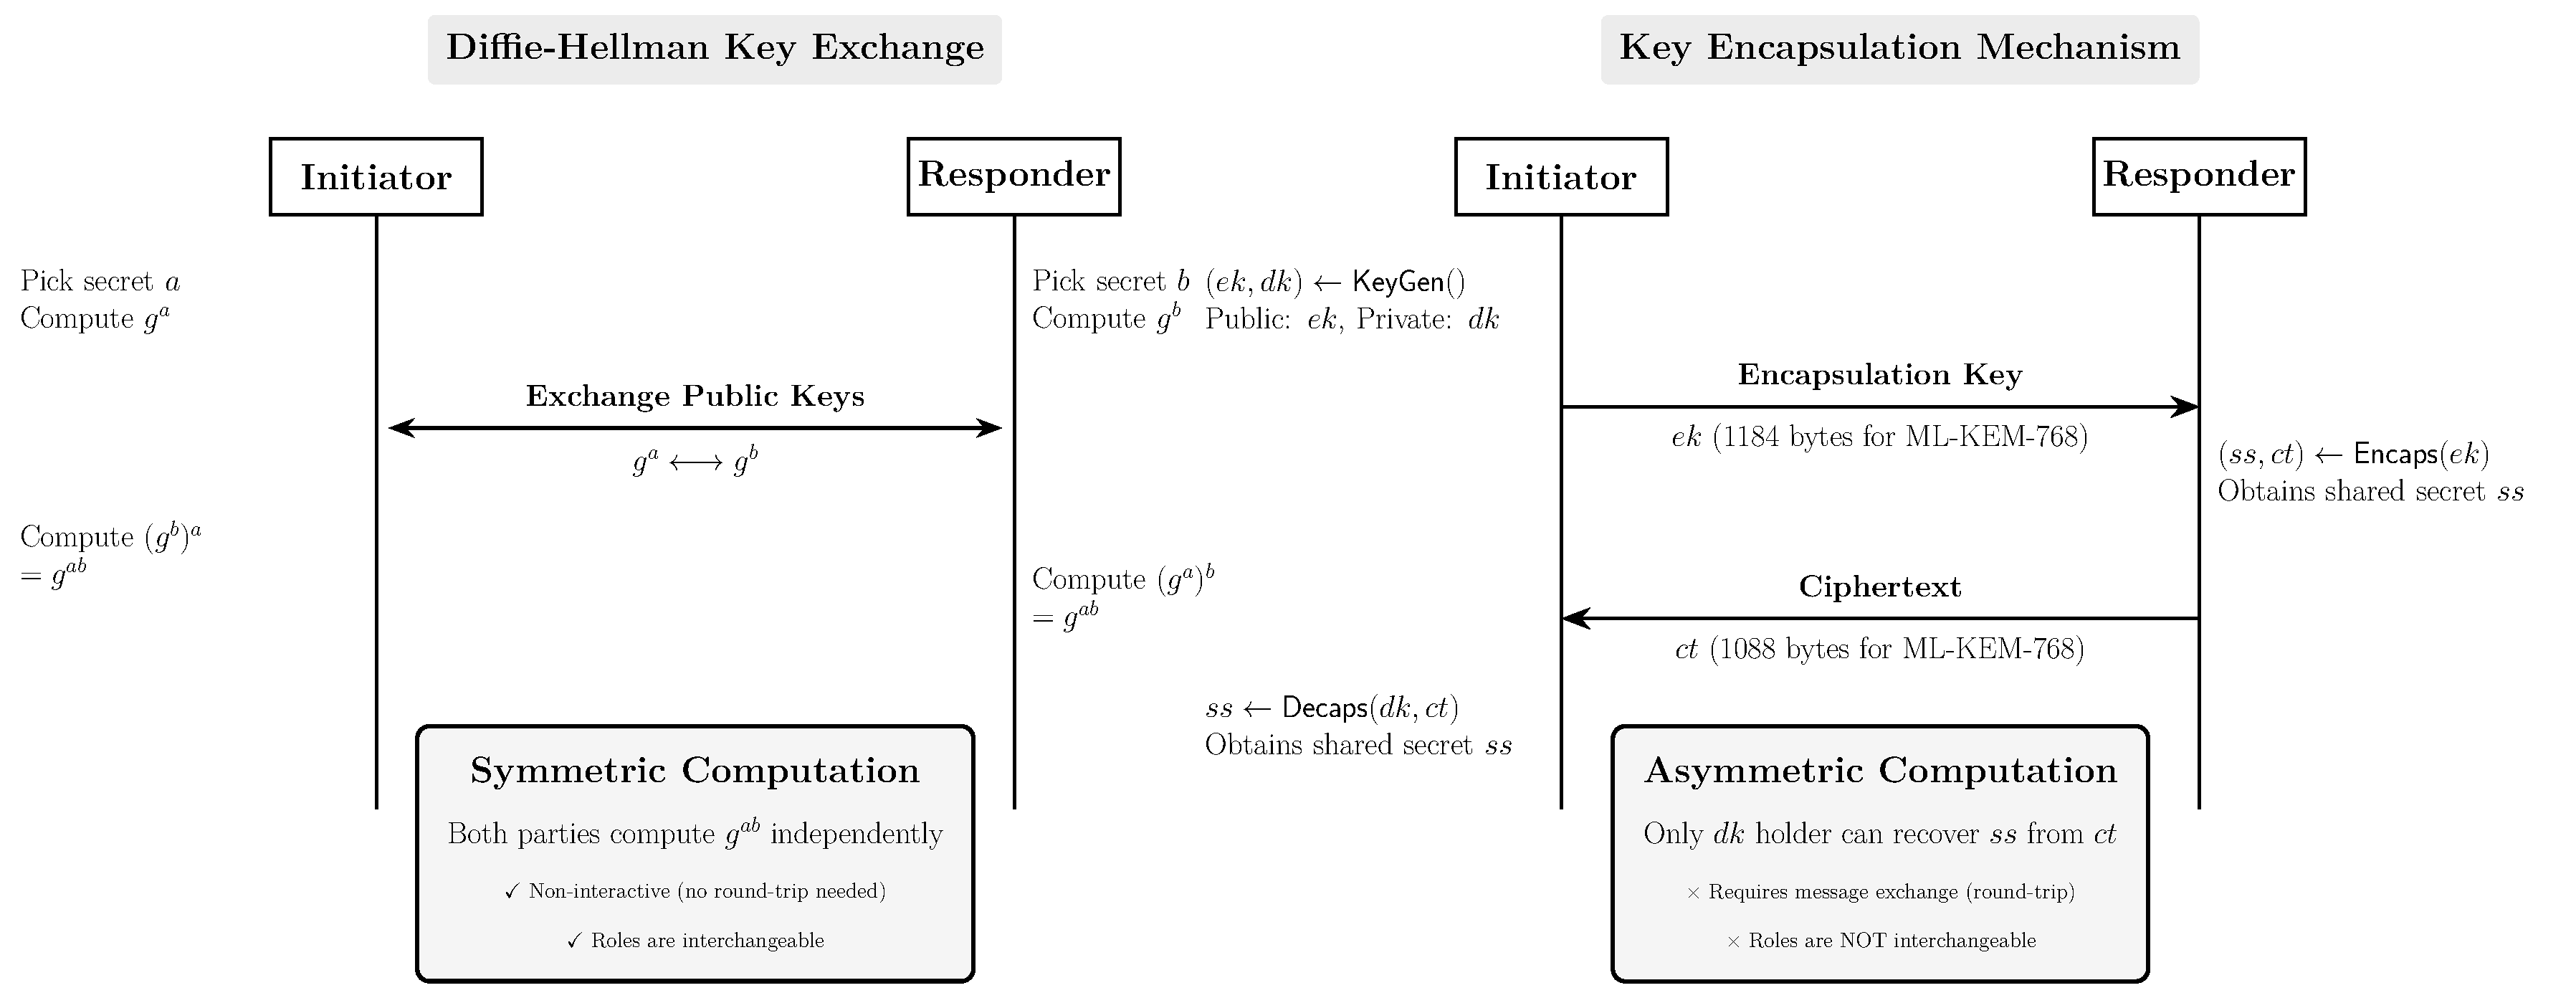
\includegraphics[width=\textwidth]{figures/fig_kem_vs_dh.pdf}
    \caption{Comparison of Diffie-Hellman key exchange and Key Encapsulation Mechanisms, illustrating the asymmetry challenge for Noise protocol migration. The KEM side shows the canonical direction, where the recipient of the shared secret publishes the encapsulation key; the hybrid construction in Chapter~\ref{chap:design} runs this the other way around, with the initiator generating an ephemeral $(\mathit{ek}, \mathit{dk})$ and sending $\mathit{ek}$ in the first message to mirror the X25519 ephemeral flow.}
    \label{fig:kem_vs_dh}
\end{figure}

\section{ML-KEM (FIPS 203)}

ML-KEM was standardized as FIPS 203 in August 2024~\cite{fips203}. It is a key encapsulation mechanism derived from CRYSTALS-Kyber~\cite{bos2018crystals}, whose 2018 EuroS\&P paper was authored by Bos, Ducas, Kiltz, Lepoint, Lyubashevsky, Schanck, Schwabe, Seiler, and Stehl\'{e}; Avanzi, Ding, and others joined the broader NIST Kyber submission team.

A KEM exposes three operations: KeyGen produces an encapsulation key and a decapsulation key; Encaps takes an encapsulation key and returns a ciphertext plus a shared secret; Decaps takes the decapsulation key and the ciphertext and recovers the same shared secret. Correctness is guaranteed as long as randomness generation is sound.

The security of ML-KEM rests on the Module Learning With Errors (MLWE) problem, introduced by Regev in 2005 and generalized to module lattices by Langlois and Stehlé~\cite{langlois2015worst}. The MLWE problem asks: given a matrix A, vectors $b = As + e$ for small error $e$ and secret $s$, distinguish $(A, b)$ from uniform random. No efficient quantum algorithm is known for this problem; the best attacks remain classical lattice reduction algorithms whose complexity scales superpolynomially with the security parameter.

ML-KEM is constructed in two steps. First, a public-key encryption scheme K-PKE is built from the MLWE problem. K-PKE is IND-CPA secure --- that is, secure against chosen-plaintext attacks --- but not IND-CCA2 secure. The IND-CCA2 security required for use in key exchange is obtained by applying a variant of the Fujisaki-Okamoto transform, which converts the PKE scheme into a KEM with the stronger security guarantee. The construction has been the target of several formal verification efforts, with machine-checked proofs of the FO transform and of Kyber-like schemes carried out in EasyCrypt and other proof assistants.

FIPS 203 specifies three parameter sets: ML-KEM-512 (NIST security category 1, equivalent to AES-128), ML-KEM-768 (category 3, equivalent to AES-192), and ML-KEM-1024 (category 5, equivalent to AES-256). The key and ciphertext sizes are as follows: ML-KEM-512 has a 800-byte encapsulation key and 768-byte ciphertext; ML-KEM-768 has a 1,184-byte encapsulation key and 1,088-byte ciphertext; ML-KEM-1024 has a 1,568-byte encapsulation key and 1,568-byte ciphertext. All three produce a 32-byte shared secret. NIST recommends ML-KEM-768 as the default parameter set, providing a large security margin at reasonable performance cost.

On the implementation side, ML-KEM benefits from the Number-Theoretic Transform (NTT), which makes polynomial multiplication efficient and gives ML-KEM a raw speed advantage over elliptic-curve operations. Benchmarks on Intel Xeon hardware show Kyber-768 key generation, encapsulation, and decapsulation each running roughly 2--3$\times$ faster than the corresponding X25519 operations in CPU cycles. In practice, though, this speed advantage is offset by the much larger key and ciphertext sizes, which tend to dominate handshake time whenever the network is the bottleneck.

\section{Hybrid Key Exchange and the Concatenate-then-KDF Pattern}

Hybrid key exchange combines two or more key agreement algorithms so that the resulting key is secure as long as at least one component holds. The motivation is straightforward: ML-KEM, though now standardized, is far newer than X25519 and has seen less cryptanalytic scrutiny. Running both in parallel means a breakthrough against either one alone does not compromise security.

The standard construction is the concatenate-then-KDF pattern, formalized in NIST SP 800-56C Rev. 2~\cite{nist-sp800-56c}. SP 800-56C explicitly permits hybrid shared secrets of the form $Z' = Z \| T$, a concatenation of a ``standard'' shared secret $Z$ (e.g., from X25519) and an auxiliary shared secret $T$ (e.g., from ML-KEM), fed into a single key derivation function. Giacon, Heuer, and Poettering~\cite{giacon2018combiners} prove that the resulting KEM is IND-CPA-secure as long as either component is IND-CPA-secure, with the bound remaining tight even when one component is completely broken.

This is the same pattern used by Cloudflare and Google in TLS 1.3 and by the IETF hybrid TLS design draft, which specifies X25519+ML-KEM hybrid groups for TLS key exchange~\cite{ietf-tls-hybrid-design}.

\chapter{Related Work}
\label{chap:related_work}

\section{PQ-WireGuard (Hülsing et al., 2021)}

The most directly relevant prior work is PQ-WireGuard by Hülsing, Ning, Schwabe, Weber, and Zimmermann~\cite{hulsing2021pqwireguard}, published at IEEE S\&P 2021. Rather than augmenting WireGuard's X25519 handshake, PQ-WireGuard replaces it entirely with a KEM-based construction. The goal was not just post-quantum confidentiality but full post-quantum authentication as well.

They instantiate the construction with Classic McEliece for static-key authentication (IND-CCA) and a passive-security variant of Saber for ephemeral key exchange (IND-CPA), chosen partly to keep handshake messages within the IPv6 minimum MTU of 1,280 bytes. Classic McEliece is code-based, so it offers security assumption diversity relative to lattice-based schemes.

Security is proved in the eCK-PFS-PSK model (adapting the classical WireGuard proof) and verified symbolically using Tamarin, establishing session-key secrecy with perfect forward secrecy.

Benchmarks show PQ-WireGuard's handshake running at roughly 0.6$\times$ the time of standard WireGuard, which makes sense given that KEM operations are computationally cheaper than ECDH at the parameter sets they evaluate. This thesis differs in three ways: it uses a hybrid construction rather than a pure post-quantum replacement, it targets NIST-standardized ML-KEM rather than pre-standardization Saber, and it works within the existing BoringTun codebase rather than a research prototype.

\section{Post-Quantum Noise (PQNoise)}

Angel, Dowling, Hülsing, Schwabe, and Weber introduced PQNoise~\cite{pqnoise2022}, a generic framework for converting Noise protocol patterns into post-quantum equivalents using KEMs. PQNoise introduces new token types, ekem and skem, to represent KEM encapsulations to ephemeral and static public keys respectively, replacing the two-letter DH tokens (ee, es, se, ss).

One of the central problems PQNoise addresses is that KEMs cannot be combined non-interactively the way DH key shares can. When the sending party owns a static key, they cannot simply compute a DH share with the other party's ephemeral key; instead, the other party must perform the encapsulation and send the ciphertext. This asymmetry sometimes requires additional round trips compared to the classical Noise patterns.

PQNoise also introduces Static-Ephemeral Entropy Combination (SEEC), a technique for hardening randomness in KEM operations to protect against weak random number generators. The security of PQNoise patterns is proved in the flexible ACCE (fACCE) model, showing that confidentiality and authenticity are preserved.

PQNoise benchmarks using Kyber-768 on a 1,000 Mbit/s network show handshake times of 31.1ms, better than classical Noise in CPU time but slower in wall-clock time due to larger messages. PQNoise is relevant to this thesis as it defines the theoretical framework within which the hybrid handshake construction sits; the WireGuard IK pattern can be viewed as a specific instantiation of a Noise pattern, and the hybrid variant described in this thesis can be understood as a variant of the pqIK pattern augmented with classical DH.

\section{A Tale of Two Worlds: Formal Hybrid-WireGuard Analysis}

Lafourcade, Mahmoud, Ruhault, and Taleb~\cite{lafourcade2025hybrid} revisited PQ-WireGuard with a thorough formal analysis using Sapic+, ProVerif, DeepSec, and Tamarin, and proposed two improvements: PQ-WireGuard$\star$ and Hybrid-WireGuard. Their analysis uncovered weaknesses in the original PQ-WireGuard, including vulnerability to Unknown-Key-Share (UKS) attacks and failure to achieve initiator/responder anonymity.

PQ-WireGuard$\star$ addresses these issues through modifications to the key derivation that incorporate both parties' static public keys, preventing the UKS attack. Hybrid-WireGuard is then constructed by combining the DH secrets from WireGuard with the KEM secrets from PQ-WireGuard$\star$ via concatenation, and formally proving that security holds as long as either the classical or post-quantum component is secure.

The paper also highlights a point directly relevant here: MTU constraints heavily limit which KEMs can be used in WireGuard, since handshake messages need to fit within the IPv6 minimum of 1,280 bytes. Their Hybrid-WireGuard implementation is provided in Rust.

This thesis builds on their results but takes a different approach in several respects: it targets NIST-standardized ML-KEM within the existing BoringTun production codebase, accepts the larger message sizes (relying on IP fragmentation rather than constraining the parameter set), and provides empirical benchmarks on real hardware.

\section{Rosenpass}

Rosenpass~\cite{rosenpass} takes the PSK-slot idea and turns it into a continuously running daemon. Written in Rust, it generates post-quantum PSKs using Classic McEliece (IND-CCA) and Kyber-512 (IND-CPA) and injects them into WireGuard's preshared key field, refreshing the PSK every two minutes~\cite{rosenpass-github}. This bounds the exposure window: at most two minutes of traffic is at risk if a PSK is compromised. The project has been formally analyzed in ProVerif and underwent a penetration test in 2024.

Structurally, Rosenpass is similar to the PSK baseline in this thesis, with the key difference being that Rosenpass runs continuously rather than performing a one-time key injection. It serves as a practical existence proof that PSK-based post-quantum WireGuard works in production.

The limitation Rosenpass shares with this thesis's PSK baseline is the lack of per-handshake forward secrecy: if the PSK used for a given session is later compromised, that session's traffic is exposed. The full hybrid approach avoids this by generating fresh ML-KEM key material inside every handshake.

\section{Hybrid Post-Quantum WireGuard via TLS PSK Delivery}

Membrey and Beyel at ExpressVPN~\cite{membrey2025expressvpn} describe a production deployment of the PSK-slot approach, using ML-KEM hybrid TLS 1.3 to deliver WireGuard PSKs through a split-service authentication architecture. The system is live across ExpressVPN's global infrastructure, adding 15--20ms to connection establishment with no steady-state throughput penalty. It is a more operationally elaborate version of the PSK-slot idea, and it demonstrates that the approach works at commercial scale.

\section{Revised PQ-WireGuard with Reinforced KEMs}

A concurrent line of work by Hashimoto, Katsumata, Niot, and Wiggers (IEEE S\&P 2026) revisits the design of PQ-WireGuard and introduces reinforced KEMs (RKEMs) as a new building block. Their construction, using a novel ML-KEM-based RKEM called Rebar, eliminates the need for Classic McEliece static keys on the server, reducing the server's public key memory requirements by 190--390x. This work addresses a major deployment concern with the original PQ-WireGuard and represents the state of the art in purely post-quantum WireGuard design~\cite{hashimoto2026rkem}.

\chapter{Problem Statement}
\label{chap:problem}

This thesis addresses the following research question: \emph{How can WireGuard's handshake be extended with hybrid post-quantum key exchange (X25519 + ML-KEM-768) while preserving its security properties and remaining viable on resource-constrained hardware?}

More concretely, this involves four subproblems:

\begin{description}[style=nextline, leftmargin=0pt]
    \item[SP1 (Handshake Integration)] How should ML-KEM-768 be integrated into the Noise IK handshake alongside X25519? What is the correct message flow, and how are the two shared secrets combined?
    
    \item[SP2 (Key Derivation)] How should the shared secrets from X25519 and ML-KEM be combined to produce the final session keys, in a way that is consistent with NIST SP 800-56C and preserves the security argument?
    
    \item[SP3 (MTU Management)] ML-KEM-768 adds 1,184 bytes (public key) and 1,088 bytes (ciphertext) to the handshake messages. How should the implementation handle handshake messages that exceed typical MTU limits?
    
    \item[SP4 (Performance)] What is the actual cost of the hybrid construction in handshake latency on Apple Silicon and ARM hardware? How does it compare to unmodified WireGuard and to the PSK-slot baseline?
\end{description}

The PSK-slot approach is implemented as a controlled comparison point---the minimal engineering intervention that provides quantum resistance against passive HNDL adversaries---so that the additional benefit of the full hybrid can be clearly quantified.

\chapter{Design}
\label{chap:design}

\section{Design Goals}

The design is guided by several principles, roughly in order of priority:

\begin{description}[style=nextline, leftmargin=0pt]
    \item[Correctness] The hybrid handshake must produce the same session keys at both endpoints and must fail securely if either component KEM fails. The correctness of the X25519 component is inherited from the existing BoringTun implementation.
    
    \item[Security] The hybrid construction must be secure against a quantum adversary as long as at least one of X25519 or ML-KEM-768 remains unbroken. It must preserve all existing WireGuard security properties: session-key secrecy, perfect forward secrecy, replay resistance, and DoS resistance.
    
    \item[Compatibility] The implementation should coexist with unmodified WireGuard peers where possible. The PSK-slot baseline achieves this by design. The full hybrid requires protocol-level negotiation or explicit configuration of both parties to use the hybrid mode.
    
    \item[Deployability] The implementation should run on BoringTun without kernel modifications, enabling deployment on any platform that supports userspace WireGuard, including embedded and IoT devices.
    
    \item[Performance] The overhead of ML-KEM operations should not dominate handshake latency at typical network speeds. Performance on Raspberry Pi 5 is treated as the binding constraint for constrained hardware.
\end{description}

\section{The PSK-Slot Baseline}

The PSK-slot approach is the minimal intervention: a standalone binary performs ML-KEM-768 key encapsulation between two peers, derives a 256-bit shared secret, and injects it into BoringTun's preshared\_key field. After that, the WireGuard handshake proceeds exactly as in the vanilla case.

Before any WireGuard session is established, the two peers run the PSK exchange out-of-band. One peer generates an ML-KEM-768 keypair and sends the encapsulation key to the other. That peer runs ML-KEM.Encaps, obtaining a ciphertext ct and a 32-byte shared secret K, then sends ct back. The first peer runs ML-KEM.Decaps to recover the same K. Both peers configure their WireGuard interface with preshared\_key = K.

\begin{figure}[!htbp]
    \centering
    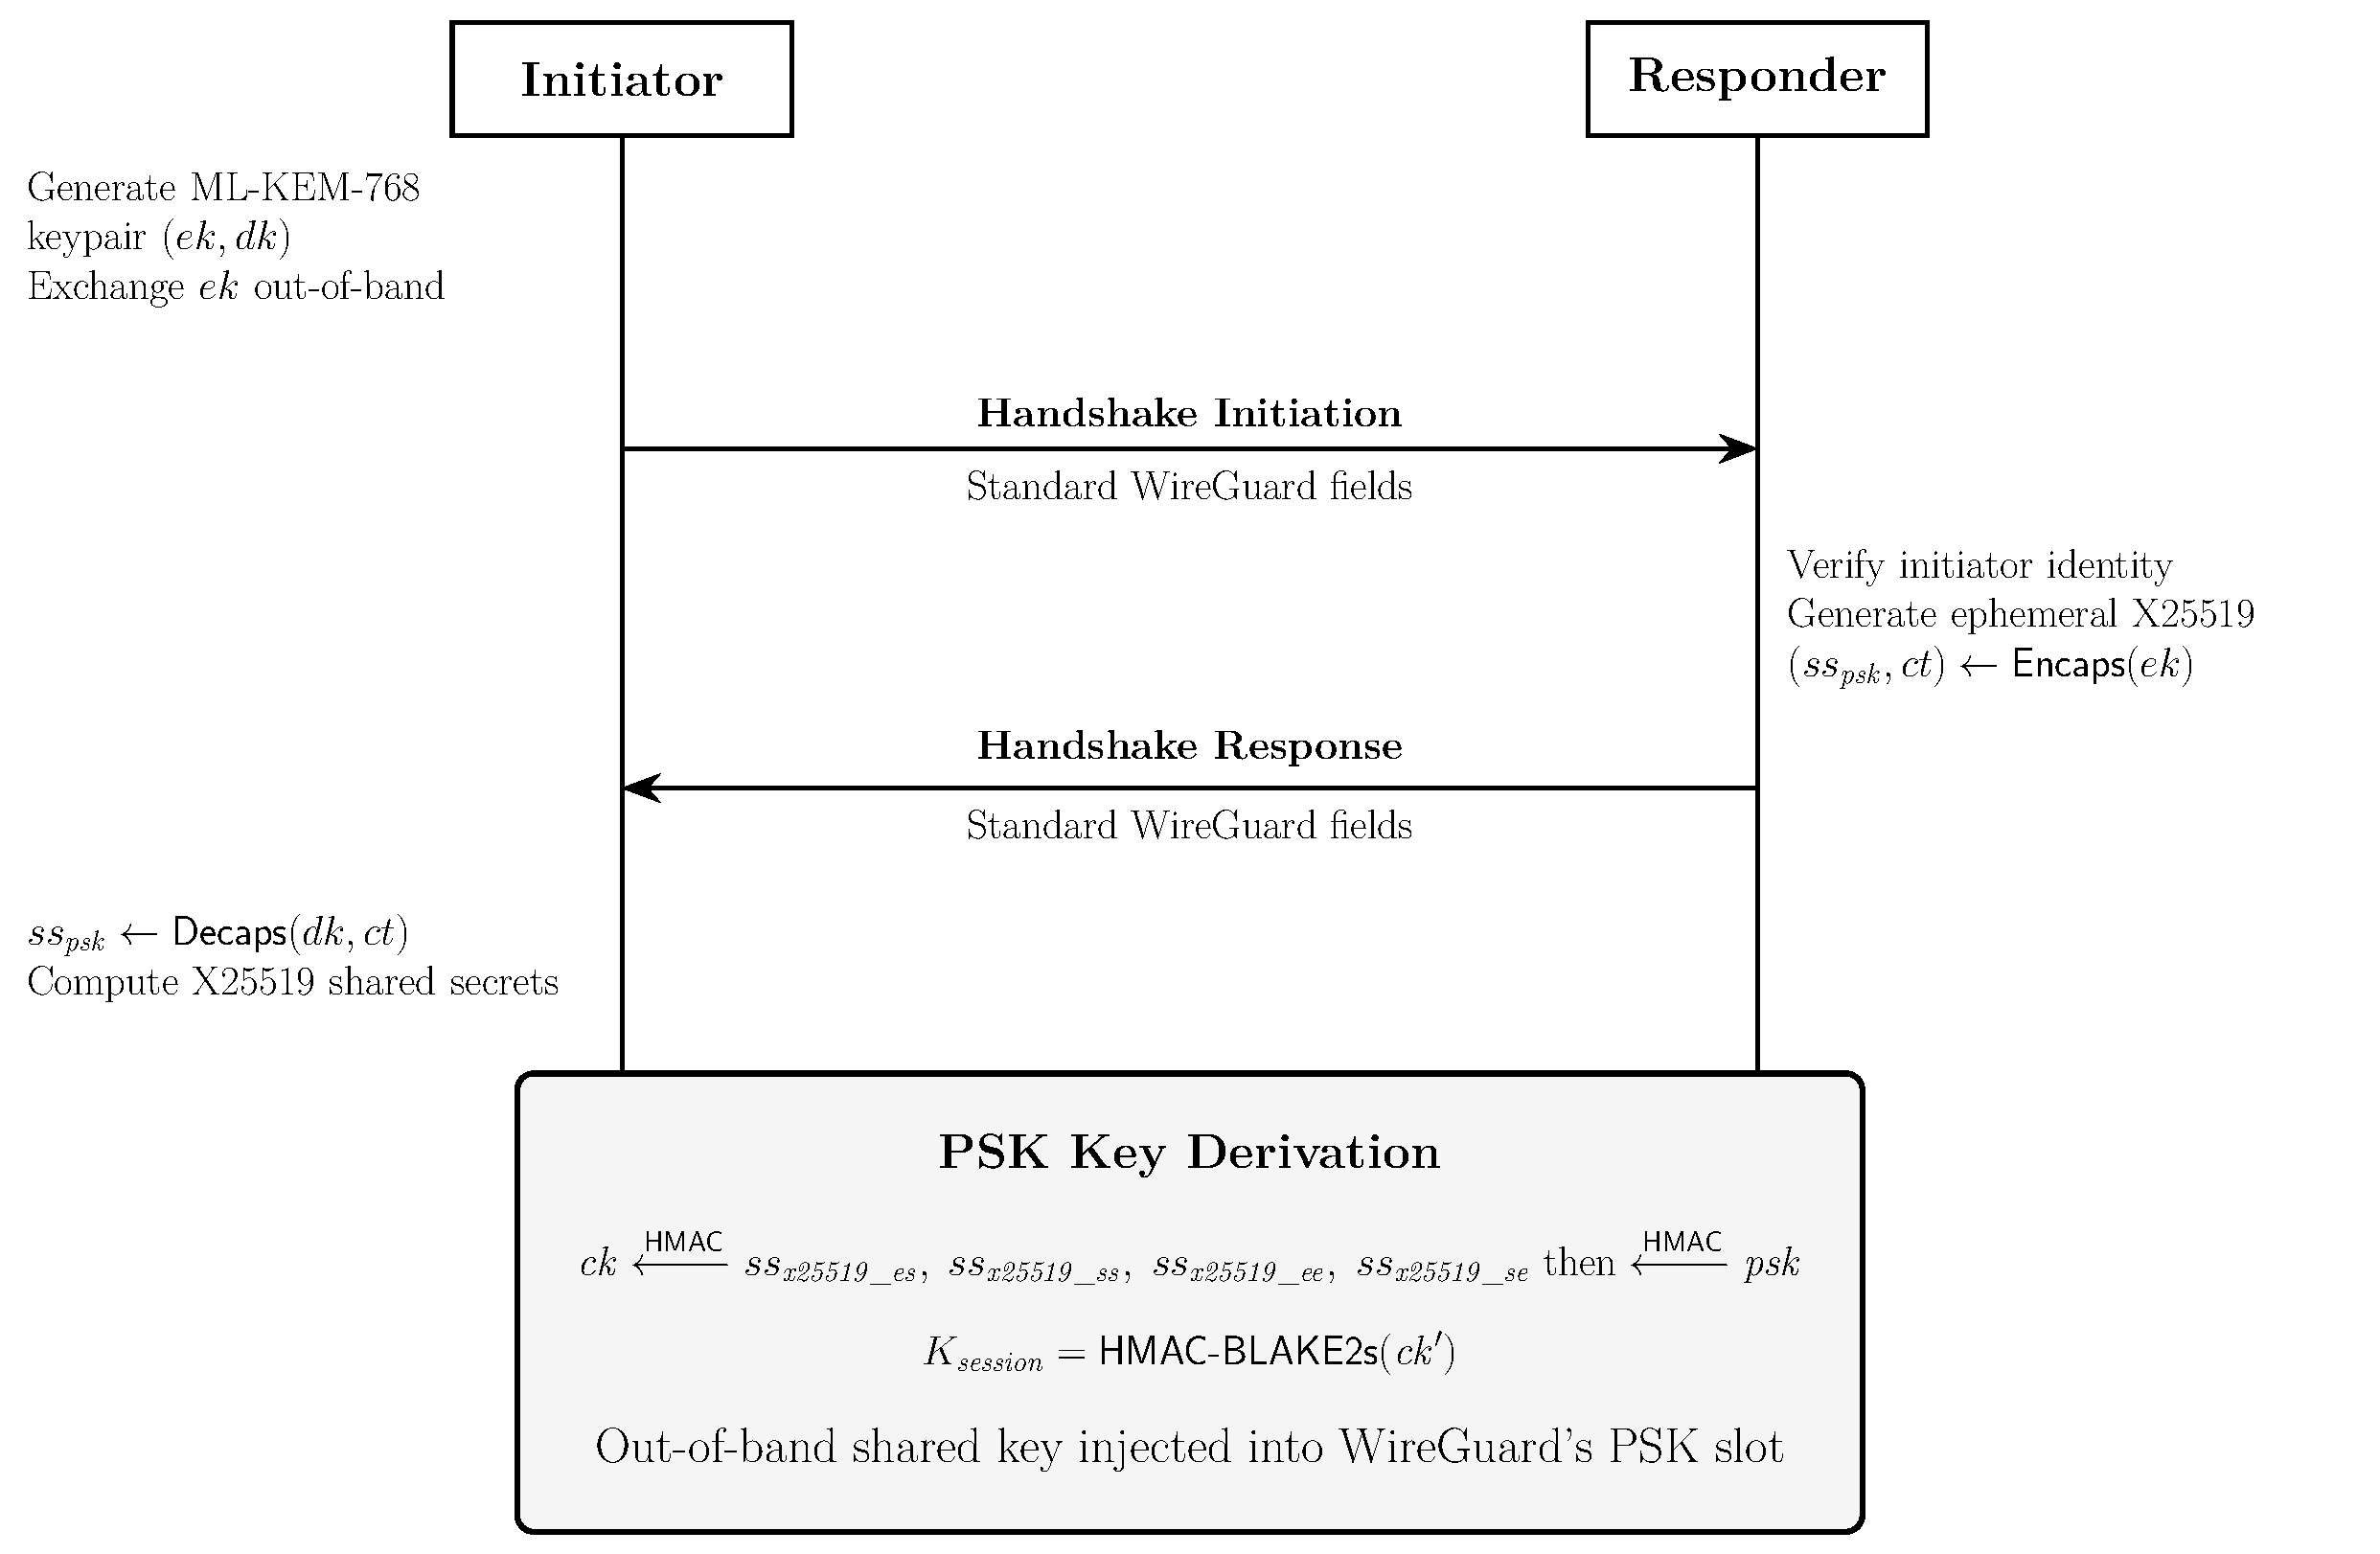
\includegraphics[width=\textwidth]{figures/fig_psk_handshake.pdf}
    \caption{PSK-Slot Baseline: Out-of-band ML-KEM exchange and PSK injection.}
    \label{fig:psk_handshake}
\end{figure}

The PSK is then mixed into the WireGuard handshake's HMAC-BLAKE2s key derivation chain, providing a quantum-resistant layer of security for all traffic protected by sessions using that PSK.

This approach has real limitations. The ML-KEM keypair used in the out-of-band exchange is static or semi-static, it does not change per handshake, so the ML-KEM component provides no forward secrecy. If the PSK is compromised after the session, all traffic from sessions that used it is exposed. The PSK also has to be distributed before any sessions can be established, which adds operational overhead.

That said, the PSK baseline has a clear advantage: it requires zero changes to WireGuard itself. It works with any existing WireGuard implementation and can be deployed immediately, providing protection against HNDL adversaries who cannot compromise the out-of-band channel.

\section{The Hybrid Handshake}

The full hybrid integrates ML-KEM-768 directly into the Noise IK handshake. The design follows the concatenate-then-KDF pattern endorsed by NIST SP 800-56C Rev.~2~\cite{nist-sp800-56c} and is structurally similar to the hybrid constructions in TLS 1.3~\cite{ietf-tls-hybrid-design}.

The modified handshake proceeds as follows:

\begin{description}[style=nextline, leftmargin=0pt]
    \item[Initiator Actions (First Message)]
    The initiator generates an ephemeral X25519 keypair as in standard WireGuard. Additionally, it generates a fresh ML-KEM-768 keypair for this session: an encapsulation key $\mathit{ek}_i$ and decapsulation key $\mathit{dk}_i$. The ML-KEM encapsulation key $\mathit{ek}_i$ (1,184 bytes) is appended to the initiator's first message, after the existing WireGuard fields. The initiator sends:
    
    \bigskip
    \begin{center}
        WireGuard initiator header, \\
        X25519 ephemeral pk, \\
        encrypted static pk, \\
        encrypted timestamp, \\
        ML-KEM-768 ek, \\
        MAC1, \\
        MAC2
    \end{center}
    \bigskip

    The ML-KEM encapsulation key is placed before the MAC fields so that MAC1 and MAC2 cover the entire message, including the ML-KEM material. This ensures that the DoS-resistance properties of the cookie mechanism extend to the post-quantum payload.

    \item[Responder Actions (Second Message)]
    The responder processes the X25519 portion of the handshake as in standard WireGuard. It also reads the initiator's ML-KEM encapsulation key $\mathit{ek}_i$ from the first message. The responder runs $\mathsf{ML\text{-}KEM.Encaps}(\mathit{ek}_i)$, producing a ciphertext $\mathit{ct}$ (1,088 bytes) and a shared secret $\mathit{ss}_\mathit{kem}$. The ciphertext $\mathit{ct}$ is appended to the responder's second message:

    \bigskip
    \begin{center}
        WireGuard responder header, \\
        X25519 ephemeral pk, \\
        encrypted empty payload, \\
        ML-KEM-768 ct, \\
        MAC1, \\
        MAC2
    \end{center}
    \bigskip

    \item[Initiator Decapsulation]
    The initiator reads $\mathit{ct}$ from the responder's message and runs $\mathsf{ML\text{-}KEM.Decaps}(\mathit{dk}_i,\allowbreak \mathit{ct})$, recovering $\mathit{ss}_\mathit{kem}$. Both peers now hold the same $\mathit{ss}_\mathit{kem}$.
    
    \item[Combined Key Derivation]
    Both parties derive the final session keys by sequentially mixing each shared secret into the Noise chaining key $\mathit{ck}$ via HMAC-BLAKE2s, following the same pattern used by standard WireGuard for its DH results. The four X25519 shared secrets from the Noise IK pattern ($\mathit{ss}_\mathit{x25519\_es}$, $\mathit{ss}_\mathit{x25519\_ss}$, $\mathit{ss}_\mathit{x25519\_ee}$, $\mathit{ss}_\mathit{x25519\_se}$, in that order) are mixed first, exactly as in vanilla WireGuard. Then the ML-KEM shared secret $\mathit{ss}_\mathit{kem}$ is mixed into $\mathit{ck}$ as an additional step:
    \[
        \mathit{temp} = \mathsf{HMAC\text{-}BLAKE2s}(\mathit{ck}, \mathit{ss}_\mathit{kem}), \quad
        \mathit{ck}' = \mathsf{HMAC\text{-}BLAKE2s}(\mathit{temp}, \mathtt{0x01})
    \]
    This sequential mixing is structurally equivalent to the concatenate-then-KDF pattern from NIST SP 800-56C Rev.~2: each shared secret contributes independently to the chaining key, and the final session keys depend on all components. The handshake hash $h$ is also updated to include the ML-KEM material (both the encapsulation key and ciphertext), binding it to the Noise transcript.
    
    \item[Transport Phase]
    After key derivation, the data transport phase proceeds identically to unmodified WireGuard. No changes are required to the ChaCha20-Poly1305 transport encryption or the session management layer.
    \end{description}

    \begin{figure}[!htbp]
    \centering
    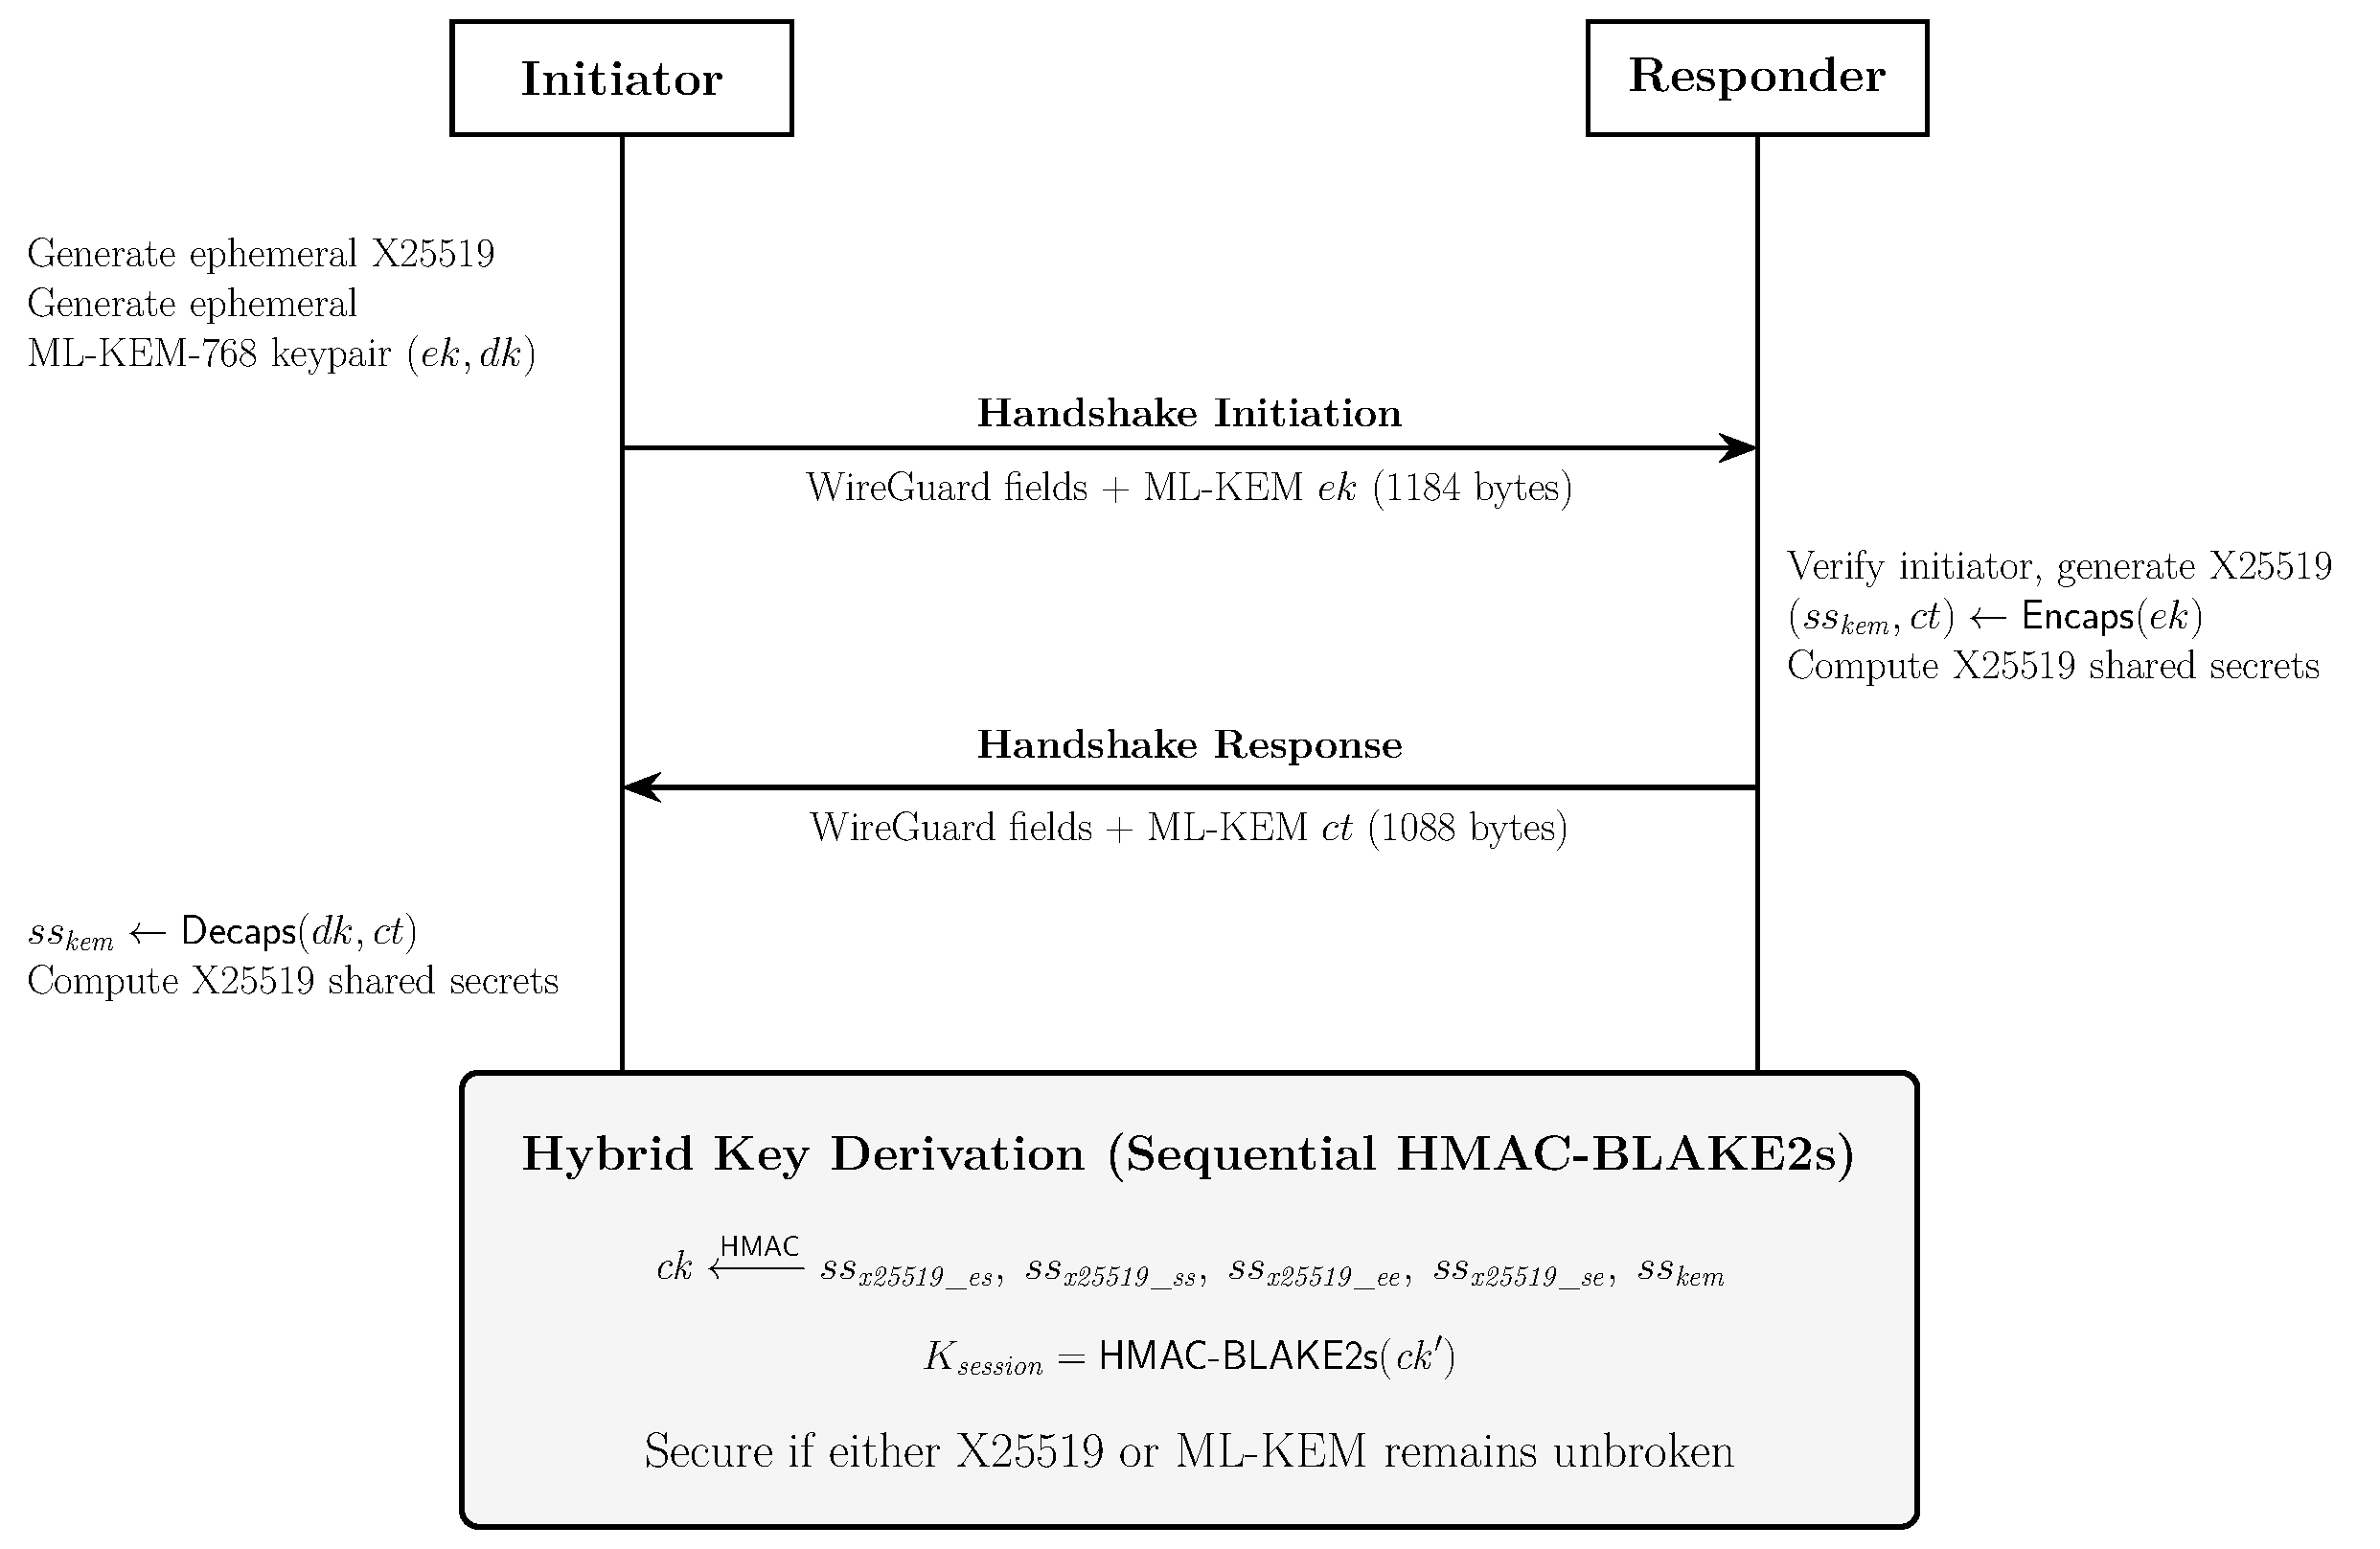
\includegraphics[width=\textwidth]{figures/fig_hybrid_handshake.pdf}
    \caption{The Full Hybrid Handshake: Integrated ML-KEM-768.}
    \label{fig:hybrid_handshake}
    \end{figure}

    Two properties follow from this design.
 Per-session forward secrecy comes from both components: the X25519 ephemeral key is fresh for each handshake, and so is the ML-KEM keypair, making $\mathit{ss}_\mathit{kem}$ unique to each session. The construction is also \emph{hybrid-secure}: if ML-KEM is completely broken (an adversary knows $\mathit{ss}_\mathit{kem}$), the session key still depends on the X25519 exchange and cannot be recovered without breaking X25519 too. The converse also holds: a quantum adversary who breaks X25519 still cannot derive the session key without also breaking ML-KEM.

\section{Key Derivation Details}

The key derivation in the hybrid handshake extends the Noise IK chaining key evolution with one additional mixing step for the ML-KEM shared secret. The approach is structurally consistent with the concatenate-then-KDF pattern from NIST SP 800-56C Rev.~2~\cite{nist-sp800-56c}, adapted to the sequential HMAC-based mixing used by the Noise Protocol Framework.

In the standard WireGuard Noise IK handshake, the chaining key $\mathit{ck}$ evolves through a sequence of HMAC-BLAKE2s mixing operations as shared secrets are established. Each DH result is mixed into $\mathit{ck}$ via a two-step HMAC extraction:
\[
    \mathit{temp} = \mathsf{HMAC\text{-}BLAKE2s}(\mathit{ck}, \mathit{ss}), \quad
    \mathit{ck} \leftarrow \mathsf{HMAC\text{-}BLAKE2s}(\mathit{temp}, \mathtt{0x01})
\]

In the hybrid, the ML-KEM shared secret $\mathit{ss}_\mathit{kem}$ is mixed into the chaining key after the X25519 DH operations and before the PSK mixing step. Concretely:

\begin{enumerate}
    \item The standard Noise IK chaining key derivation proceeds: $\mathit{ck}$ is updated with the four X25519 DH results from the IK pattern --- $\mathit{ss}_\mathit{x25519\_es}$ (ephemeral-static), $\mathit{ss}_\mathit{x25519\_ss}$ (static-static), $\mathit{ss}_\mathit{x25519\_ee}$ (ephemeral-ephemeral), and $\mathit{ss}_\mathit{x25519\_se}$ (static-ephemeral) --- each via the HMAC-BLAKE2s extraction above, exactly as in standard WireGuard. One detail worth noting: BoringTun caches $\mathit{ss}_\mathit{x25519\_ss}$ as \texttt{NoiseParams.static\_shared} when a peer is first added and reuses it across handshakes. The value is still mixed into $\mathit{ck}$ every time, but only the other three DH results are recomputed per handshake, so the per-handshake cost across both peers comes out at six fresh DH operations rather than eight (see Section~\ref{sec:handshake_latency_results}).

    \item An additional HMAC-BLAKE2s mixing step incorporates $\mathit{ss}_\mathit{kem}$:
    \[
        \mathit{temp} = \mathsf{HMAC\text{-}BLAKE2s}(\mathit{ck}, \mathit{ss}_\mathit{kem}), \quad
        \mathit{ck}' = \mathsf{HMAC\text{-}BLAKE2s}(\mathit{temp}, \mathtt{0x01})
    \]
    The ML-KEM ciphertext is also mixed into the handshake hash: $h \leftarrow \mathsf{BLAKE2s}(h \| \mathit{ct})$, binding it to the Noise transcript.

    \item The PSK mixing step proceeds on $\mathit{ck}'$ exactly as in standard WireGuard (using a zero PSK if none is configured).

    \item The final session key pair ($\mathit{send\_key}$, $\mathit{recv\_key}$) is derived from the resulting chaining key as in standard WireGuard.
\end{enumerate}

BLAKE2s is used throughout: for the handshake hash $h$, and as the PRF underlying the HMAC-based key derivation chain. This is consistent with BoringTun's existing implementation and with the WireGuard protocol specification. No SHA-256 or separate HKDF construction is introduced; the hybrid extension reuses the same HMAC-BLAKE2s extraction pattern already used for the X25519 shared secrets.

\section{Message Size Analysis and MTU Considerations}

The biggest practical challenge with the hybrid handshake is the increased message size. Vanilla WireGuard's handshake initiation message is 148 bytes and the response is 92 bytes (accounting for all headers, encrypted fields, and MACs). Adding ML-KEM-768 material adds 1,184 bytes to the initiation message (the encapsulation key) and 1,088 bytes to the response message (the ciphertext). The total handshake message sizes become approximately 1,332 bytes for the initiation and 1,180 bytes for the response.

The IPv6 minimum MTU is 1,280 bytes. Both hybrid handshake messages exceed this threshold. The IPv4 minimum MTU is 68 bytes (though in practice the de facto minimum for internet paths is 576 bytes), and typical deployed MTUs are 1,500 bytes for Ethernet.

This creates a fragmentation problem. WireGuard transmits handshake messages as UDP datagrams. Unlike TCP, UDP does not have a built-in fragmentation and reassembly mechanism at the application layer; IP-level fragmentation may occur, but it is unreliable on many real-world network paths (some firewalls drop fragments), and it reduces resilience.

The current implementation relies on IP-level fragmentation to handle oversized handshake messages. On typical Ethernet paths with a 1,500-byte MTU, the initiation message (1,332 bytes) fits in a single UDP datagram without fragmentation. The response message (1,180 bytes) also fits comfortably. On paths with a reduced MTU (e.g., the IPv6 minimum of 1,280 bytes), the initiation message will be fragmented at the IP layer. This approach is the simplest and works correctly on network paths that do not drop fragments.

For deployments on paths where IP fragmentation is unreliable (e.g., certain firewall configurations or middleboxes that drop fragments), two alternative strategies are identified as future work:

\begin{description}[style=nextline, leftmargin=0pt]
    \item[Application-Level Segmentation]
    Split the handshake messages at the application layer, sending the ML-KEM material in a separate UDP datagram. This requires a protocol extension and adds an additional round trip for ML-KEM key material exchange.

    \item[Path MTU Discovery with KEM Parameter Negotiation]
    Use PMTUD to discover the path MTU before the handshake and choose a KEM parameter set whose ciphertext fits within the available space. For most internet paths with a 1,500-byte MTU, ML-KEM-768 fits comfortably; for IPv6 paths requiring sub-1,280-byte packets, a reduced parameter set or segmentation would be needed.
\end{description}

These strategies are not implemented in the current version of the hybrid handshake. On standard 1,500-byte MTU paths the IP-level approach already does the job, and a proper quantitative study of how the hybrid behaves on constrained paths is left as future work.

\chapter{Implementation}
\label{chap:implementation}

\section{BoringTun Architecture}

BoringTun~\cite{boringtun} is Cloudflare's userspace WireGuard implementation, written in Rust and deployed on millions of iOS and Android devices along with thousands of Cloudflare Linux servers. It ships as a library crate (\texttt{boringtun}) and a CLI binary (\texttt{boringtun-cli}). The library handles the WireGuard protocol itself but leaves networking and tunnel management to the application layer.

The part of BoringTun that matters for this thesis is the handshake module, which implements the Noise IK pattern. It manages per-peer handshake state machines, performs X25519 operations via the x25519-dalek crate (already a dependency), and uses HMAC-BLAKE2s for chaining key evolution and key derivation. The transport module (ChaCha20-Poly1305 encryption and decryption) is not touched.

Being written in Rust helps here. The ownership and borrowing model rules out buffer overflows, use-after-free, and double-free bugs at compile time, which matters for cryptographic code where such bugs have historically led to exploitable vulnerabilities. It also makes it easy to pull in pure-Rust cryptographic crates from the RustCrypto ecosystem without introducing C FFI boundaries.

\section{Technology Stack}

The implementation relies on the following dependencies:

\textbf{ML-KEM:} The ml-kem crate (version 0.3.0-rc.0) from RustCrypto, a pure-Rust, \texttt{no\_std} implementation of FIPS 203. It supports all three ML-KEM parameter sets and is tested against the NIST Known Answer Test (KAT) vectors. Being pure Rust and \texttt{no\_std} means it runs on constrained targets like the Raspberry Pi without needing any C FFI.

\textbf{X25519:} The x25519-dalek crate is already a dependency of BoringTun and is used for the existing X25519 operations. No changes are required.

\textbf{Key derivation:} HMAC-BLAKE2s is used for chaining key evolution and key derivation, consistent with WireGuard's specification and BoringTun's existing implementation. No separate HKDF or SHA-256 construction is introduced; the hybrid extension reuses the same HMAC-BLAKE2s extraction pattern already present in BoringTun.

\textbf{Test hardware:} Apple MacBook Pro M4 (Apple Silicon, ARM64) and Raspberry Pi 5 (Cortex-A76, ARM64).

\textbf{RNG compatibility:} The ml-kem crate needs \texttt{rand\_core} 0.10, but BoringTun already depends on \texttt{rand\_core} 0.6. Cargo's package renaming feature resolves this: \texttt{rand\_core\_pq} (aliasing \texttt{rand\_core} 0.10) and \texttt{getrandom\_pq} (aliasing \texttt{getrandom} 0.4) are declared as separate optional dependencies, letting both versions coexist in the same binary.

\section{Handshake Module Modifications}

The primary implementation change is to BoringTun's handshake module. All post-quantum code is conditionally compiled behind a Cargo feature flag (\texttt{pq}), ensuring that vanilla builds are completely unaffected: no additional dependencies are compiled, no code paths change, and binary size remains identical. The \texttt{pq} feature gates the ml-kem, rand\_core\_pq, and getrandom\_pq dependencies, as well as all PQ-related message types, state fields, and handshake methods. The following modifications are made when the feature is enabled:

\textbf{State structure extension:} The HandshakeState structure is extended with fields for the ML-KEM ephemeral keypair. On the initiator side, an ml\_kem\_768::\allowbreak EncapsulationKey and ml\_kem\_768::\allowbreak DecapsulationKey are stored. On the responder side, the received encapsulation key (parsed from the initiation message) and the encapsulated ciphertext (to be included in the response message) are stored.

\textbf{Initiation message construction:} When the initiator constructs the handshake initiation message, it generates a fresh ML-KEM-768 keypair (ml\_kem\_768::KeyGen()) and appends the 1,184-byte encapsulation key after the standard WireGuard fields. The encapsulation key is added to the handshake hash h via BLAKE2s mixing, binding it to the Noise transcript.

\textbf{Response message construction:} When the responder processes the initiation message, it extracts the ML-KEM encapsulation key, validates its length, and runs ml\_kem\_768::Encaps() to produce a ciphertext ct and shared secret ss\_kem. The 1,088-byte ciphertext is appended after the standard WireGuard response fields and mixed into the handshake hash.

\textbf{Session key derivation:} At the end of the handshake, both parties mix ss\_kem into the chaining key via one additional HMAC-BLAKE2s extraction step before proceeding to the PSK mixing and final session key derivation. On the initiator side, ss\_kem is obtained by running ml\_kem\_768::Decaps() on the received ciphertext. A new error variant (\texttt{MlKemDecapsulationFailed}) is added to handle decapsulation failures gracefully, causing the handshake to abort without leaking state.

\textbf{New message types:} Two new message types are introduced: type 5 for PQ handshake initiation (1,332 bytes) and type 6 for PQ handshake response (1,180 bytes). The packet parser dispatches on message type and size, routing PQ messages to the corresponding PQ handshake methods. Vanilla builds (without the \texttt{pq} feature) reject these message types with \texttt{InvalidPacket}, ensuring graceful interoperability.

\textbf{MTU handling:} The current implementation relies on IP-level fragmentation for oversized handshake messages. On typical Ethernet paths with a 1,500-byte MTU, both hybrid messages fit in a single UDP datagram. Application-level segmentation and Path MTU Discovery are identified as future work for deployment on paths where IP fragmentation is unreliable.

\section{PSK-Slot Baseline Implementation}

The PSK-slot baseline is implemented as a separate Rust CLI binary, \texttt{pq-psk-tool}, that operates independently of BoringTun. It uses the same ml-kem crate (version 0.3.0-rc.0). The binary provides three subcommands that implement a manual three-step ML-KEM-768 key exchange:

\begin{enumerate}
    \item \texttt{pq-psk-tool keygen}: Generates an ML-KEM-768 keypair. The encapsulation key (1,184 bytes) is written as a base64-encoded file for transfer to the peer. The decapsulation key seed (64 bytes) is written as a separate base64 file and kept secret.
    \item \texttt{pq-psk-tool encaps <ek\_file>}: Reads the peer's encapsulation key, runs ML-KEM.Encaps, and outputs both the ciphertext (as a base64 file for transfer back to the peer) and the 32-byte shared secret (as a hex-encoded PSK file).
    \item \texttt{pq-psk-tool decaps <dk\_file> <ct\_file>}: Reads the local decapsulation key seed and the peer's ciphertext, runs ML-KEM.Decaps, and recovers the identical 32-byte PSK.
\end{enumerate}

The key and ciphertext files are exchanged out-of-band using any secure channel available to the operator (e.g., \texttt{scp}, USB transfer, or a secure messaging channel). The tool itself does not implement a network protocol; it is a purely local utility that reads and writes files. Both peers then configure their WireGuard interface with the derived PSK using \texttt{wg set <iface> peer <PUBKEY> preshared-key psk.hex}.

This is deliberately minimal: no networking code, no daemon, just file I/O. The choice of how to securely move files between peers is left to the operator. For production deployments that need automated PSK distribution, pairing with a daemon like Rosenpass~\cite{rosenpass} or a TLS-protected channel as described by Membrey and Beyel~\cite{membrey2025expressvpn} would make more sense.

\section{Test Harness}

The test infrastructure consists of two components: unit tests within the BoringTun crate and a shell-based integration test script.

\subsection{Unit Tests}

The \texttt{noise::tests} module in BoringTun contains tests for both vanilla and PQ handshake paths, conditionally compiled with \texttt{\#[cfg(\allowbreak feature = "pq")]} and \texttt{\#[cfg(not(\allowbreak feature = "pq"))]}:

\begin{itemize}
\item \textbf{PQ handshake message validation:} Verifies that the PQ initiation message is exactly 1,332 bytes (type 5) and the PQ response is exactly 1,180 bytes (type 6), and that both parse correctly.

\item \textbf{Full PQ handshake:} Exercises the complete four-step exchange (init, response, keepalive, done) and verifies that both peers derive working session keys.

\item \textbf{End-to-end data transport:} Performs a full PQ handshake, then encrypts and decrypts an IPv4 UDP packet, verifying that the decrypted payload matches the original.

\item \textbf{PQ with PSK:} Validates that the hybrid ML-KEM handshake and the traditional PSK mechanism can be used simultaneously, confirming their orthogonality.

\item \textbf{PSK-slot baseline:} Tests the PSK-slot approach by configuring both tunnels with a shared 32-byte PSK (simulating the output of \texttt{pq-psk-tool}), performing a full handshake and data exchange. A companion test verifies that mismatched PSKs cause handshake failure.

\item \textbf{Vanilla rejects PQ:} Verifies that a vanilla build (without the \texttt{pq} feature) rejects PQ message types with \texttt{InvalidPacket}, confirming graceful interoperability.
\end{itemize}

\subsection{Integration Test Script}

A shell script (\texttt{pq-hybrid-test.sh}) automates operational testing on macOS. It provides several modes:

\begin{itemize}
\item \textbf{Demo mode:} Displays PQ vs.\ vanilla packet sizes and runs unit tests for both configurations.

\item \textbf{Local tunnel mode:} Creates two BoringTun peers on loopback interfaces, performs a PQ hybrid handshake, and verifies end-to-end connectivity via ping. Handshake logs are inspected to confirm type 5/6 message exchange.

\item \textbf{Comparison mode:} Runs vanilla and PQ hybrid tunnels side-by-side on separate interfaces and ports, verifying that both configurations achieve successful connectivity.
\end{itemize}

All measurements are taken on the Apple MacBook Pro M4 (local loopback) and on a Raspberry Pi 5 (local loopback and network link between the two machines). Results are compared across all three configurations (vanilla, PSK-slot, hybrid).

\chapter{Security Analysis}
\label{chap:security}

\section{Security Goals}

The security goals for the hybrid handshake are the same as for vanilla WireGuard, as established by Dowling and Paterson's computational proof~\cite{dowling2018wireguard} and Donenfeld and Milner's symbolic Tamarin proof~\cite{donenfeld2018formal}, and extended to the post-quantum setting by PQ-WireGuard~\cite{hulsing2021pqwireguard} and Hybrid-WireGuard~\cite{lafourcade2025hybrid}:

\textbf{Session-key secrecy:} A passive or active adversary who does not corrupt either party's long-term or ephemeral secrets cannot distinguish the established session key from a random value.

\textbf{Perfect forward secrecy (PFS):} Compromise of long-term static keys does not allow an adversary to decrypt past sessions. This holds because each session uses a fresh ephemeral keypair (both X25519 and ML-KEM), so past session keys cannot be derived from the static keys alone.

\textbf{Post-quantum forward secrecy:} The X25519 PFS guarantee is extended to the quantum setting: a quantum adversary who breaks X25519 after the session cannot decrypt past traffic, because doing so also requires breaking ML-KEM, which remains computationally hard.

\textbf{Authenticity:} Both the initiator and responder can verify each other's identity via their static public keys (X25519 static keys, as in standard WireGuard). Authentication is classical, not post-quantum, in this design.

\textbf{DoS resistance:} The existing WireGuard cookie mechanism is preserved. Handshake initiation messages with invalid MAC1 are rejected without server state allocation, maintaining the DoS resistance property of vanilla WireGuard.

\textbf{Replay resistance:} The Noise handshake transcript, extended to include the ML-KEM material, prevents replay attacks. The handshake hash h binds all transmitted material, including the ML-KEM ciphertext, to the session.

\section{Hybrid Security Argument}

The security of the hybrid construction follows from the concatenate-then-KDF security proof. Let $\mathit{ss}_\mathit{classical}$ denote the combined X25519 shared secrets derived from the Noise IK exchange, and let $\mathit{ss}_\mathit{kem}$ denote the ML-KEM-768 shared secret. The chaining key $\mathit{ck}$ evolves through sequential HMAC-BLAKE2s mixing of each shared secret. After the classical exchange, $\mathit{ck}$ already incorporates $\mathit{ss}_\mathit{classical}$. The ML-KEM shared secret is then mixed in:

\begin{equation}
\mathit{ck}' = \mathsf{HMAC\text{-}BLAKE2s}(\mathsf{HMAC\text{-}BLAKE2s}(\mathit{ck}, \mathit{ss}_\mathit{kem}), \mathtt{0x01})
\end{equation}

The session keys $K$ are derived from $\mathit{ck}'$ after the PSK mixing step.

\textbf{Claim:} $K$ is computationally indistinguishable from a random key as long as either $\mathit{ss}_\mathit{classical}$ is pseudorandom (i.e., X25519 is secure) OR $\mathit{ss}_\mathit{kem}$ is pseudorandom (i.e., ML-KEM-768 is IND-CCA2 secure).

This follows from the security of HMAC-BLAKE2s as a PRF: if either input to the chaining key is a uniformly random value independent of the adversary's view, then the chaining key output, and consequently the derived session keys, are computationally indistinguishable from random (under the assumption that BLAKE2s is a secure PRF). The sequential mixing of independent shared secrets into the chaining key is structurally equivalent to the concatenate-then-KDF pattern, as each component contributes independently to the final key material. The formal proof is a standard hybrid argument; Giacon, Heuer, and Poettering~\cite{giacon2018combiners} give it for the concatenation combiner.

In the HNDL threat model, the adversary captures the handshake transcript, which includes both the X25519 public keys and the ML-KEM ciphertext ct. With a quantum computer, the adversary can recover ss\_classical from the X25519 keys. However, to recover ss\_kem, the adversary must also solve the ML-KEM decapsulation problem — specifically, recover the ML-KEM private key dk\_i from the public encapsulation key ek\_i and then decapsulate ct. This is the IND-CCA2 security problem for ML-KEM, which is believed computationally hard for both classical and quantum adversaries under the MLWE assumption.

\section{Forward Secrecy Analysis}

The hybrid handshake provides genuine per-session forward secrecy for the ML-KEM component, in contrast to the PSK-slot baseline.

In the PSK-slot baseline, the ML-KEM exchange is performed once, out-of-band, and the resulting PSK is reused across many WireGuard sessions. If an adversary compromises the PSK after the fact — through the out-of-band channel, key theft, or other means — all sessions using that PSK are retroactively vulnerable, even to a purely classical adversary. The ML-KEM component does not contribute ephemeral, per-session material.

In the full hybrid, the ML-KEM keypair (ek\_i, dk\_i) is generated fresh for every WireGuard handshake. The ciphertext ct encapsulates ss\_kem specifically for that session's ephemeral public key ek\_i. Once the session key has been derived and dk\_i has been zeroed from memory (consistent with WireGuard's existing practice of zeroing ephemeral keys after use), there is no remaining information that would allow recovery of ss\_kem. An adversary who subsequently breaks into either peer's memory finds no material that compromises past sessions.

This makes the hybrid's forward secrecy against quantum adversaries equivalent in structure to X25519's forward secrecy against classical adversaries: in both cases, the ephemeral key is gone, and the session key cannot be reconstructed.

\section{Authentication and Remaining Limitations}

An important limitation of this design, shared with most practical hybrid WireGuard proposals, is that authentication stays classical. The static public keys used for identity binding in the Noise IK pattern are X25519 keys. A quantum adversary with a large enough quantum computer could, in principle, compute the static private key from the static public key and impersonate either party in new sessions. However:

\begin{enumerate}
\item Authentication cannot be retroactively broken: even if a quantum adversary eventually recovers the static X25519 key, it cannot retroactively forge the authentication in past sessions, because authentication affects only the handshake transcript, not the session data.

\item The HNDL threat for past sessions is mitigated by the ML-KEM component in the hybrid: even with the static X25519 key, an adversary cannot reconstruct past session keys without breaking ML-KEM (for sessions using the hybrid handshake).

\item Future work could extend the authentication layer to use ML-DSA (FIPS 204) for post-quantum signatures, but this significantly increases complexity and is outside the scope of this thesis.
\end{enumerate}

The hybrid design also inherits WireGuard's identity-hiding properties: the initiator's static public key is encrypted before transmission and is not visible to passive eavesdroppers. Whether this identity hiding extends fully to the post-quantum setting, and whether it can be formally proved along the lines of the Hybrid-WireGuard analysis, is left as future work.

\section{Comparison of the Two Approaches}

The PSK-slot baseline and the full hybrid differ in three important ways:

\textbf{Forward secrecy for the quantum component:} The hybrid provides per-handshake ephemeral ML-KEM exchange, giving full post-quantum forward secrecy. The PSK-slot approach does not.

\textbf{Protocol transparency:} The PSK-slot approach works with any WireGuard implementation; it requires no changes to the WireGuard protocol. The hybrid requires both peers to use a modified WireGuard implementation and to agree to use the hybrid mode.

\textbf{Operational complexity:} The PSK-slot approach requires a separate key exchange infrastructure and periodic PSK rotation (or uses a static PSK, reducing security). The hybrid integrates key exchange into the WireGuard handshake automatically, with no additional infrastructure.

For deployments where engineering effort is at a premium and forward secrecy for the quantum component is not required, the PSK-slot approach is appropriate. For deployments handling sensitive long-lived data where the full HNDL threat model applies, the hybrid is strongly preferable.

\chapter{Evaluation}
\label{chap:evaluation}

This chapter evaluates the hybrid handshake along three axes: handshake latency, transport throughput, and primitive-level microbenchmarks. All measurements were collected on two platforms that sit at opposite ends of the ARM64 performance spectrum:

\begin{itemize}
    \item \textbf{Apple MacBook Pro M4 (Apple Silicon):} ARMv8.5-A, 14-core, 24GB RAM,\\macOS Tahoe. The development machine itself, and the high-performance reference.

    \item \textbf{Raspberry Pi 5 (Broadcom BCM2712, Cortex-A76):} ARM64, 4-core, 8GB RAM, Raspberry Pi OS Lite (64-bit). A common choice for embedded or edge deployments and a reasonable stand-in for resource-constrained environments.
\end{itemize}

\noindent Three configurations are compared:

\begin{itemize}
    \item \textbf{Vanilla:} Unmodified BoringTun, no PSK.

    \item \textbf{PSK-slot:} BoringTun with a WireGuard PSK derived from a one-time ML-KEM-768 exchange via \texttt{pq-psk-tool}.

    \item \textbf{Hybrid:} The modified BoringTun with the full X25519 + ML-KEM-768 hybrid handshake.
\end{itemize}

One practical detail worth noting: the \texttt{pq} Cargo feature is a compile-time switch. When the binary is built with \texttt{--features pq}, \emph{all} tunnels go through the hybrid handshake path (there is no runtime toggle). So the vanilla and PSK-slot baselines come from a separate build without that feature flag, while the hybrid numbers come from a PQ-enabled build. Each data point is from a different binary, which has the side benefit that cache and branch-predictor state never crosses configurations.

All the microbenchmarks here (the handshake one, the ML-KEM ops, and the X25519 ops) are driven by Criterion~\cite{criterion}, which handles warm-up per benchmark, throws out outliers, and reports bootstrapped 95\% confidence intervals. For the handshake bench specifically, two \texttt{Tunn} instances exchange bytes in-process via function calls on the same machine, with no sockets or OS scheduler in the loop, so the measurement reflects pure cryptographic cost. Inside the non-PQ binary, vanilla and PSK-slot are registered in a random order on every run (a coin flip from the OS RNG), so even if there is any residual ordering bias it averages out across repeated invocations. Each configuration is measured with Criterion's sample size set to 500: that is 500 measurement samples after warm-up, each itself a batch of handshake iterations. For transport throughput, \texttt{iperf3} is used in two setups: M4 loopback (both BoringTun instances on the same host, talking over 127.0.0.1) and cross-device (Mac to Pi over local Wi-Fi, through a real WireGuard tunnel).

\section{Handshake Latency Results}
\label{sec:handshake_latency_results}

\begin{table}[H]
\centering
\caption{Handshake latency across configurations and platforms (loopback, Criterion sample size 500). Each cell shows the bootstrapped per-iteration point estimate followed by the 95\% CI.}
\label{tab:handshake_latency}
\begin{tabular}{@{}llr@{}}
\toprule
\textbf{Configuration} & \textbf{Platform} & \textbf{Latency ($\mu$s, [95\% CI])} \\
\midrule
Vanilla   & M4              & 150.82 [150.70, 150.94] \\
PSK-slot  & M4              & 150.99 [150.86, 151.12] \\
Hybrid    & M4              & 247.34 [247.06, 247.63] \\
\midrule
Vanilla   & Raspberry Pi 5  & 1312.2 [1312.1, 1312.3] \\
PSK-slot  & Raspberry Pi 5  & 1311.5 [1311.4, 1311.6] \\
Hybrid    & Raspberry Pi 5  & 1642.9 [1642.7, 1643.1] \\
\bottomrule
\end{tabular}
\end{table}

On the M4, the hybrid handshake adds about 97~$\mu$s over vanilla, a 64\% increase. The sum of the isolated ML-KEM operations (KeyGen + Encaps + Decaps $\approx$ 73~$\mu$s, from Table~\ref{tab:mlkem_benchmarks}) accounts for most of that overhead, with the remaining $\sim$24~$\mu$s coming from the extra work the handshake has to do around the KEM: an extra BLAKE2s pass over the encapsulation key and ciphertext (which together add 2,272 bytes to the transcript), the extra HMAC-BLAKE2s mixing step for $\mathit{ss}_\mathit{kem}$, and the larger heap buffers needed to hold the PQ messages. As for PSK-slot, it sits inside vanilla's 95\% confidence interval; the gap is a fraction of a microsecond and changes sign between runs, which is what you would expect given that PSK mixing only adds a handful of HMAC-BLAKE2s calls. The earlier methodology made it look spuriously \emph{faster} than vanilla because both configurations ran from a single warm-up loop and PSK-slot benefited from caches that vanilla had already primed; with Criterion's per-benchmark warm-up and the randomised registration order, that artefact is gone.

The Pi tells a somewhat different story. The hybrid adds about 331~$\mu$s on top of vanilla, a 25\% increase. The three ML-KEM operations together account for $\sim$280~$\mu$s of that gap (Table~\ref{tab:mlkem_benchmarks}), and the remaining $\sim$51~$\mu$s is mostly the cost of moving the PQ payloads through the handshake: the PQ messages are around 1.3~KB and 1.2~KB versus 148~B and 92~B for the classical path, and the extra BLAKE2s passes plus the larger heap buffers cost more on the Cortex-A76's narrower memory subsystem than on the M4. The Pi numbers for vanilla and PSK-slot are within a microsecond of each other (1312.2~$\mu$s vs 1311.5~$\mu$s); at a 1.3~ms baseline that gap is well below any practically meaningful threshold, even though Criterion's CIs are tight enough to make them not formally overlap, and the sign of the gap has also flipped from one run to the next during testing.

It is also worth noting that on the Pi, the classical handshake is overwhelmingly dominated by X25519. A single DH operation takes 192.81~$\mu$s (Table~\ref{tab:mlkem_benchmarks}), and the IK pattern mixes four DH results into the chaining key on each side (\emph{es}, \emph{ss}, \emph{ee}, \emph{se}). BoringTun caches the static-static $\mathit{ss}$ once per peer and reuses it across handshakes (see Chapter~\ref{chap:design}), so only three of the four are recomputed per peer per handshake --- six fresh DH operations across both peers. That alone accounts for $\sim$1157~$\mu$s of the 1312.2~$\mu$s vanilla figure, with another $\sim$116~$\mu$s going to the two ephemeral key generations. Only about 39~$\mu$s is left for everything else (BLAKE2s, ChaCha20-Poly1305, bookkeeping). The ML-KEM operations simply add on top of this X25519-dominated baseline.

A caveat: the loopback setup measures cryptographic cost only. It does not capture the time to actually push the larger PQ messages across a network link. In practice, handshake latency over a real connection is dominated by RTT, not by the sub-millisecond difference between configurations, so this limitation does not change the overall picture.

\section{Handshake Packet Sizes}

\begin{table}[H]
\centering
\caption{Handshake packet sizes for each configuration.}
\label{tab:packet_sizes}
\begin{tabular}{@{}lrrr@{}}
\toprule
\textbf{Configuration} & \textbf{Initiation (bytes)} & \textbf{Response (bytes)} & \textbf{Total (bytes)} \\
\midrule
Vanilla   & 148       & 92        & 240 \\
PSK-slot  & 148       & 92        & 240 \\
Hybrid    & 1,332 & 1,180 & 2,512 \\
\bottomrule
\end{tabular}
\end{table}

The PSK-slot numbers are identical to vanilla because the PSK never appears in the handshake messages, it is mixed into the key derivation chain locally on each peer. The hybrid, on the other hand, must carry the ML-KEM encapsulation key in the initiation (+1,184 bytes) and the ciphertext in the response (+1,088 bytes), for 2,272 bytes of additional handshake traffic. These sizes are fixed by the ML-KEM-768 specification and do not vary between runs.

\section{Transport Throughput}

\begin{table}[H]
\centering
\caption{Transport throughput after handshake completion (\texttt{iperf3}, $t = 15$\,s).}
\label{tab:throughput}
\begin{tabular}{@{}llr@{}}
\toprule
\textbf{Configuration} & \textbf{Setup} & \textbf{Throughput (Mbps)} \\
\midrule
Vanilla & M4 loopback             & 489 \\
Hybrid  & M4 loopback             & 491 \\
\midrule
Vanilla & M4 $\rightarrow$ Raspberry Pi 5  & 78.6 \\
Hybrid  & M4 $\rightarrow$ Raspberry Pi 5  & 77.5 \\
\bottomrule
\end{tabular}
\end{table}

The numbers are essentially the same across configurations, as expected. The 2~Mbps gap on loopback and the 1.1~Mbps gap cross-device are well within normal \texttt{iperf3} run-to-run variance. On the M4 loopback, the $\sim$490~Mbps figure is CPU-bound: BoringTun has to encrypt and decrypt every packet in userspace with ChaCha20-Poly1305 and shuttle it through a TUN device and UDP socket, which saturates a single core. Over Wi-Fi, the $\sim$78~Mbps reflects the link speed, not the Pi's crypto capacity. The Cortex-A76 handles the workload comfortably at that rate.

This table functions as a sanity check more than a performance claim. All three configurations use the same ChaCha20-Poly1305 data plane once the handshake is done, so throughput parity is the only reasonable outcome; any difference would point to an implementation bug rather than a fundamental cost. A Pi-only loopback test was not included because the Linux kernel routes traffic between two WireGuard interfaces on the same host directly, bypassing encryption entirely; without network namespaces to force real encapsulation, the measurements would not be reliable.

\section{ML-KEM Operation Benchmarks}

To understand where the handshake overhead actually comes from, each cryptographic primitive was measured in isolation. Both the ML-KEM-768 and X25519 operations now go through Criterion with a sample size of 1000, so the microbenchmark numbers are all produced the same way (per-operation warm-up, outlier detection, bootstrapped 95\% confidence intervals) and are directly comparable.

\begin{table}[H]
\centering
\caption{ML-KEM-768 and X25519 operation microbenchmarks (Criterion, point estimate followed by 95\% CI).}
\label{tab:mlkem_benchmarks}
\begin{tabular}{@{}lrr@{}}
\toprule
\textbf{Operation} & \textbf{M4 ($\mu$s, [95\% CI])} & \textbf{Raspberry Pi 5 ($\mu$s, [95\% CI])} \\
\midrule
ML-KEM-768 KeyGen & 24.13 [24.10, 24.16] & 81.66 [81.65, 81.67]    \\
ML-KEM-768 Encaps & 20.82 [20.80, 20.85] & 82.77 [82.76, 82.77]    \\
ML-KEM-768 Decaps & 28.03 [27.99, 28.07] & 115.15 [115.14, 115.16] \\
\midrule
X25519 KeyGen     & 8.77 [8.76, 8.78]    & 58.00 [57.99, 58.00]    \\
X25519 DH         & 20.39 [20.36, 20.41] & 192.81 [192.80, 192.82] \\
\bottomrule
\end{tabular}
\end{table}

The relative performance of ML-KEM and X25519 depends heavily on the platform. On the M4, the two primitives end up roughly comparable on a per-operation basis: X25519 DH and ML-KEM Encaps are within half a microsecond of each other (20.39~$\mu$s vs 20.82~$\mu$s), ML-KEM Decaps is the slowest single op at 28.03~$\mu$s, and the only place where X25519 clearly wins is keypair generation, at 8.77~$\mu$s against 24.13~$\mu$s for ML-KEM KeyGen, a $\sim$2.75$\times$ gap. On the Pi, the relationship flips. X25519 DH balloons to 192.81~$\mu$s, while ML-KEM KeyGen and Encaps sit around 82~$\mu$s and Decaps at 115~$\mu$s, all of them clearly cheaper than a single DH. The likely reason is that the \texttt{x25519-dalek} implementation BoringTun uses does not take advantage of NEON vectorisation on the Cortex-A76, while ML-KEM's NTT-based arithmetic maps well onto the integer pipeline.

The eBACS reference figures from the background chapter (X25519 $\sim$135k cycles vs Kyber-768 KeyGen $\sim$40k, Encaps $\sim$54k, Decaps $\sim$42k, measured on Intel Xeon) predicted that ML-KEM would be 2--3$\times$ faster than X25519. The M4 results don't quite line up with that: X25519 DH and ML-KEM Encaps end up roughly tied, probably because the M4's wide out-of-order core handles both workloads close to peak. The Pi numbers, however, broadly agree: X25519 DH at 192.81~$\mu$s is about 2.3$\times$ slower than ML-KEM Encaps at 82.77~$\mu$s on the Cortex-A76.

Putting this back in context of the full handshake: the three ML-KEM operations together cost about 73~$\mu$s on the M4, roughly 48\% of a vanilla handshake. The measured hybrid overhead from Table~\ref{tab:handshake_latency} is about 64\%, so the ML-KEM ops account for most of the gap and the remaining $\sim$16 percentage points come from the handling around them: the extra BLAKE2s pass, the bigger buffers, the extra mixing step. On the Pi, the KEM cost ($\sim$280~$\mu$s) is about 21\% of the vanilla handshake while the measured hybrid overhead is around 25\%, leaving roughly four percentage points (about 51~$\mu$s) for the same per-message bookkeeping. That is consistent with the M4 picture, just scaled differently relative to the much larger X25519 baseline on the Pi.

\section{ML-KEM Parameter Set Sweep}
\label{sec:mlkem_param_sweep}

The hybrid implementation in this thesis pins ML-KEM-768, but FIPS-203 defines three parameter sets: ML-KEM-512 (NIST level 1), ML-KEM-768 (level 3), and ML-KEM-1024 (level 5). Picking between them is a three-way tradeoff between security margin, per-handshake compute cost, and on-wire message size. The compute side of that tradeoff was measured by running the same Criterion harness against all three sets on each platform.

\begin{table}[H]
\centering
\caption{ML-KEM operation latency across all three FIPS-203 parameter sets and platforms (Criterion, sample size 1000, point estimate followed by 95\% CI).}
\label{tab:mlkem_param_sweep}
\begin{tabular}{@{}llrrr@{}}
\toprule
\textbf{Param set} & \textbf{Platform} & \textbf{Keygen ($\mu$s)} & \textbf{Encaps ($\mu$s)} & \textbf{Decaps ($\mu$s)} \\
\midrule
ML-KEM-512  & M4              & 14.40 [14.39, 14.41]    & 12.71 [12.69, 12.72]    & 17.50 [17.48, 17.53]    \\
ML-KEM-512  & Raspberry Pi 5  & 48.32 [48.29, 48.38]    & 51.64 [51.64, 51.65]    & 74.70 [74.70, 74.71]    \\
ML-KEM-512  & Ryzen 7 5700X   & 20.94 [20.89, 21.00]    & 20.27 [20.22, 20.33]    & 28.88 [28.81, 28.96]    \\
\midrule
ML-KEM-768  & M4              & 23.85 [23.82, 23.87]    & 21.26 [21.21, 21.32]    & 27.99 [27.93, 28.06]    \\
ML-KEM-768  & Raspberry Pi 5  & 81.61 [81.60, 81.62]    & 84.04 [84.03, 84.04]    & 116.39 [116.28, 116.62] \\
ML-KEM-768  & Ryzen 7 5700X   & 35.83 [35.75, 35.93]    & 33.88 [33.76, 34.01]    & 45.54 [45.43, 45.66]    \\
\midrule
ML-KEM-1024 & M4              & 36.84 [36.79, 36.89]    & 31.15 [31.13, 31.17]    & 40.79 [40.75, 40.84]    \\
ML-KEM-1024 & Raspberry Pi 5  & 125.61 [125.60, 125.63] & 127.80 [127.78, 127.81] & 167.42 [167.41, 167.43] \\
ML-KEM-1024 & Ryzen 7 5700X   & 56.09 [55.97, 56.23]    & 51.41 [51.27, 51.57]    & 66.44 [66.29, 66.59]    \\
\bottomrule
\end{tabular}
\end{table}

The scaling between security levels is roughly linear in NIST category on all three platforms: going from ML-KEM-512 to ML-KEM-1024 (a 2$\times$ jump in category) costs about 2.5$\times$ more per op, give or take. So the parameter-set choice does not buy or cost order-of-magnitude factors of latency, and at handshake scale (microseconds, not milliseconds) any of the three is well within the budget that the X25519 baseline already sets on every platform. ML-KEM-1024 on the Pi is the worst case in the table, at 167~$\mu$s for Decaps, which is still cheaper than a single X25519 DH at 192.81~$\mu$s on the same hardware.

\begin{table}[H]
\centering
\caption{Hybrid handshake datagram sizes by ML-KEM parameter set, holding the rest of the wire format fixed. The encapsulation key is carried in the initiation and the ciphertext in the response.}
\label{tab:hybrid_msg_sizes_by_param}
\begin{tabular}{@{}lrrrr@{}}
\toprule
\textbf{Param set} & \textbf{EK (B)} & \textbf{CT (B)} & \textbf{Hybrid init (B)} & \textbf{Hybrid response (B)} \\
\midrule
ML-KEM-512  &  800 &  768 &  948 &  860 \\
ML-KEM-768  & 1184 & 1088 & 1332 & 1180 \\
ML-KEM-1024 & 1568 & 1568 & 1716 & 1660 \\
\bottomrule
\end{tabular}
\end{table}

Where the choice actually matters is the wire. The 1280-byte IPv6 minimum MTU is the load-bearing threshold: only ML-KEM-512 fits under it without IP-level fragmentation. At a standard 1500-byte Ethernet MTU, both ML-KEM-512 and ML-KEM-768 fit comfortably; ML-KEM-1024's 1716-byte initiation always fragments. Picking ML-KEM-768 (as the thesis implementation does) gives NIST level 3 while remaining unfragmented on any normal Ethernet path; falling back to ML-KEM-512 is the only way to stay below the IPv6 floor; moving up to ML-KEM-1024 buys level-5 security at the cost of guaranteed fragmentation on every link. That is the empirical picture the parameter-set agility discussion in Chapter~\ref{chap:discussion} hangs on.

\chapter{Discussion}
\label{chap:discussion}

\section{Choosing Between the PSK-Slot and Hybrid Approaches}

The PSK-slot and hybrid approaches are not just different implementations of the same idea; they occupy genuinely different positions in the security/complexity tradeoff space. For operators who need post-quantum protection today with minimal disruption, the PSK-slot approach is the pragmatic choice. It requires no WireGuard code changes, works with any existing client and server, and can be rolled out incrementally. Rosenpass and ExpressVPN's PSK-over-TLS deployment show this works at scale~\cite{rosenpass,membrey2025expressvpn}.

The hybrid approach makes more sense when the threat model includes not just passive HNDL adversaries but also future active attackers with quantum computers. Its key advantage is per-handshake forward secrecy: every WireGuard session gets a fresh ML-KEM keypair, so even if key material is somehow compromised after the fact, past sessions remain protected. With the PSK-slot approach, a single PSK compromise can expose months of traffic.

Looking further ahead, the hybrid is better aligned with where things are going. Organizations facing the 2030 or 2035 NIST deprecation deadlines will eventually need a WireGuard deployment whose key exchange is fully quantum-resistant without depending on external key management. The PSK-slot approach defers that problem; the hybrid solves it.

\section{Deployment Considerations}

Beyond the security analysis, several practical issues affect whether the hybrid handshake can actually be deployed:

\textbf{MTU management} is the most pressing operational concern. Network paths with an effective MTU below roughly 1,360 bytes --- the 1,332-byte initiation plus its IP and UDP headers --- will fragment the hybrid initiation message. Fragmentation is not universally supported: firewalls, middleware boxes, and some ISP configurations drop IP fragments. The current implementation relies on IP-level fragmentation, which works on most standard Ethernet paths (1,500-byte MTU). For deployment on paths where fragmentation is unreliable, future work could implement application-level segmentation (splitting ML-KEM material into separate datagrams) or Path MTU Discovery with KEM parameter negotiation. One thing that does \emph{not} help, despite being the obvious first reflex, is lowering the WireGuard interface MTU: that shrinks the encapsulated data packets, not the fixed-size handshake messages, so the fragmentation has to be solved in the handshake itself.

\textbf{Interoperability} is a constraint: both endpoints must run the hybrid-capable BoringTun. A vanilla WireGuard peer will reject the extended handshake messages outright: the post-quantum message types (5 and 6) are unrecognized, so the packet is dropped as invalid at type dispatch, before MAC verification is ever attempted. Some form of capability negotiation --- a reserved field in the handshake, or simply an out-of-band configuration flag --- would be needed for gradual rollout. This is an engineering problem, not a fundamental one.

\textbf{Key management} is actually simpler with the hybrid than with the PSK-slot approach. X25519 static keys are managed as before, and the ML-KEM ephemeral keys are generated and discarded within each handshake. There is nothing new to distribute or rotate.

\textbf{Performance on constrained hardware} matters for edge and IoT deployments. The Raspberry Pi 5 benchmarks (Chapter~\ref{chap:evaluation}) are intended as a proxy for ARM-based edge devices, and the picture they paint is encouraging: the hybrid handshake overhead on the Pi is sub-millisecond, well below the RTT of any realistic WAN path, so at this hardware tier handshake cost is dominated by the network rather than by ML-KEM computation. The footprint matches: turning the hybrid on adds only about 65~KiB of code and a fraction of a megabyte of peak memory (Table~\ref{tab:footprint}), small enough to be a non-issue well below the Pi's hardware tier.

\section{Authentication Agility and Future Work}

Authentication in this thesis remains classical (X25519 static keys), which means it is quantum-vulnerable. A future version could extend the authentication layer to ML-DSA (FIPS 204) for post-quantum signatures, or use static ML-KEM keys for authentication as PQ-WireGuard and Hybrid-WireGuard do. Either option significantly increases key management complexity (ML-DSA-65 public keys, the security-level match for ML-KEM-768, are 1,952 bytes, compared to 32 bytes for X25519) and may require rethinking how WireGuard keys are distributed.

Leaving authentication classical is a deliberate choice, consistent with NIST's guidance~\cite{nistir8547} that key agreement migration (where HNDL attacks apply) is more urgent than signature migration (where past signatures cannot be retroactively forged). Key exchange is what the 2030/2035 deadline targets.

\textbf{Rosenpass integration:} A natural extension of the PSK-slot baseline is to integrate with the Rosenpass daemon, which continuously refreshes the WireGuard PSK using post-quantum key exchange. The combination of Rosenpass-managed PSKs and the hybrid handshake would provide layered post-quantum security: the handshake ML-KEM provides ephemeral forward secrecy, and the Rosenpass PSK provides additional quantum-resistant keying material. However, careful analysis is needed to confirm that double-layering does not introduce new vulnerabilities.

\textbf{Formal verification:} The informal security argument in this thesis should be supplemented by a formal proof in a computational model. The eCK-PFS-PSK model used by Hülsing et al.\ for PQ-WireGuard~\cite{hulsing2021pqwireguard}, and the Sapic+-based approach of Lafourcade et al.\ for Hybrid-WireGuard~\cite{lafourcade2025hybrid}, provide templates for how such a proof would be structured.

\textbf{Parameter set agility:} The implementation currently targets ML-KEM-768. An extension could allow negotiation between ML-KEM-512 (smaller messages, NIST level 1) and ML-KEM-1024 (larger messages, NIST level 5) based on the available path MTU and the security requirements of the deployment.

\textbf{MTU fragmentation handling:} The current implementation relies on IP-level fragmentation for paths with MTUs below roughly 1,360 bytes (the 1,332-byte initiation plus IP and UDP headers). Two alternative strategies merit investigation: application-level segmentation, where the ML-KEM material is sent in a separate UDP datagram (adding a round trip but avoiding IP fragmentation), and Path MTU Discovery with KEM parameter negotiation, where the handshake selects an ML-KEM parameter set (e.g., ML-KEM-512 for constrained paths) that fits within the discovered MTU. Both approaches add protocol complexity and would require careful design to avoid introducing downgrade attacks.

\textbf{Crypto-agility concerns:} WireGuard's deliberate lack of cipher agility is a security strength — it prevents protocol downgrade attacks of the kind that have plagued TLS. The hybrid implementation should not introduce algorithm negotiation that could be exploited for downgrade attacks. The recommended approach is to configure the ML-KEM parameter set at the operator level, not to negotiate it per-connection.

\section{Positioning within the Broader PQ-WireGuard Landscape}

It is worth being clear about where this thesis sits relative to the existing work, since it differs from prior efforts in a few important ways. Most academic PQ-WireGuard proposals are built on prototype implementations; this work targets a production Rust codebase already running on millions of devices. It commits to NIST-standardized ML-KEM (FIPS 203), rather than the pre-standardization or alternative primitives used by earlier efforts --- Saber and McEliece in PQ-WireGuard, Kyber before standardization in Rosenpass. And it is deliberately hybrid, pairing X25519 with ML-KEM so that a break in either primitive still leaves the session protected, whereas PQ-WireGuard is purely post-quantum.

The construction also differs. For the full hybrid, the Noise handshake is modified directly, rather than carrying the post-quantum secret through the PSK slot as Rosenpass and ExpressVPN do. The evaluation, in turn, spans two ARM hardware tiers (though the implementation is not ARM-specific and would run well on x86\_64 too), which makes the measurements in Chapter~\ref{chap:evaluation} directly relevant to the constrained, edge-class deployments this work targets.

The closest academic work is the Hybrid-WireGuard proposal of Lafourcade et al.~\cite{lafourcade2025hybrid}; the two are complementary rather than overlapping. Their work proves a hybrid protocol secure, while this thesis implements one in a production codebase and measures its cost. Their proofs are the formal counterpart to the informal argument made here.

\chapter{Conclusions}
\label{chap:conclusions}

This thesis has presented a hybrid post-quantum key exchange for WireGuard, integrating ML-KEM-768 alongside X25519 in the Noise IK handshake. The implementation targets BoringTun, Cloudflare's production Rust userspace WireGuard, and to our knowledge is the first FIPS 203-compliant hybrid WireGuard prototype built on a real-world codebase.

The core idea is straightforward: the initiator sends its ML-KEM encapsulation key in the first handshake message, the responder returns the ciphertext in the second, and both shared secrets (X25519 and ML-KEM) are mixed sequentially into the Noise chaining key via HMAC-BLAKE2s. This is structurally consistent with the NIST SP 800-56C concatenate-then-KDF pattern and gives a hybrid-secure construction: security holds as long as at least one of the two components remains unbroken. Because the ML-KEM keypair is generated fresh for every handshake, the hybrid also provides post-quantum forward secrecy, which the PSK-slot baseline cannot.

The PSK-slot baseline, implemented as a small companion CLI tool, serves as a comparison point. It is simpler to deploy and works with unmodified WireGuard, but it lacks per-session forward secrecy for the quantum component.

On the engineering side, the main challenge is the larger handshake messages: ML-KEM-768 adds about 2,272 bytes total. The current implementation handles this through IP-level fragmentation, which works on standard Ethernet paths. Application-level segmentation and path-MTU-aware strategies are left as future work. Empirical evaluation on Apple M4 and Raspberry Pi 5 shows that the ML-KEM computation itself is the dominant source of overhead, with the larger handshake messages adding a smaller secondary cost, and that transport throughput is unaffected.

With NIST's 2030 deprecation deadline for classical key exchange approaching~\cite{nistir8547} and the harvest-now-decrypt-later threat no longer hypothetical, post-quantum key exchange for VPN protocols is becoming an operational requirement rather than a research exercise. This thesis offers a practical starting point for WireGuard's migration, built on NIST standards and tested on hardware that spans high-performance and resource-constrained environments.


% Bibliography
\cleardoublepage
\bibliography{references}

\end{document}
